\documentclass[../FinalThesis.tex]{subfiles}
\begin{document}
\chapter{Dispersal and Connectivity in Increasingly Extreme Climatic Conditions}
\label{ChapterFlood}
\thispagestyle{empty}
\vspace{-1cm}
\noindent\hfil\rule{0.75\textwidth}{.4pt}\hfil

\begin{center}
David D. Hofmann \orcid{0000-0003-3477-4365},
Dominik M. Behr \orcid{0000-0001-7378-8538},
John W. McNutt,
Arpat Ozgul \orcid{0000-0001-7477-2642}, and
Gabriele Cozzi \orcid{0000-0002-1744-1940}

% \begin{flushleft}

% \vspace{5cm}
\vfill

Published in Global Change Biology (2024):
\url{https://doi.org/10.1111/gcb.17299}.

% \textsuperscript{1} Department of Evolutionary Biology and Environmental
% Studies, University of Zurich, Winterthurerstrasse 190, 8057 Zurich,
% Switzerland.
%
% \vspace{0.25cm}
%
% \textsuperscript{2} Botswana Predator Conservation Program, Wild Entrust,
% Private Bag 13, Maun, Botswana.
%
% \vspace{0.25cm}
%
% \textsuperscript{\S} Corresponding author:
% \href{mailto:david.hofmann2@uzh.ch}{david.hofmann2@uzh.ch}

\end{center}

% \vfill

% \textbf{Running Title:}\\African Wild Dog Dispersal in a Changing Climate:
% Lessons Learned from Seasonal Flood Extremes
%
% \vspace{0.5cm}
%
% \textbf{Keywords:}\\movement, connectivity, climate change, seasonality,
% dispersal, conservation, individual-based simulations, step-selection

% \end{flushleft}

\newpage
\section*{Abstract}
While climate change has been shown to impact several life-history traits of
wild-living animal populations, little is known about its effects on dispersal
and connectivity.

Here, we capitalize on the highly variable flooding regime of the Okavango Delta
to investigate impacts of changing environmental conditions on dispersal and
connectivity of the endangered African wild dog (\textit{Lycaon pictus}). Based
on remote sensed flood extents observed over 20 years, we derive two extreme
flood scenarios: a minimum and a maximum flood extent; representative of very
dry and very wet environmental periods. These conditions are akin to those
anticipated under increased climatic variability, as it is expected under
climate change. Using a movement model parametrized with GPS data from
dispersing individuals, we simulate 12,000 individual dispersal trajectories
across the ecosystem under both scenarios and investigate patterns of
connectivity.

Across the entire ecosystem, surface water coverage during maximum flood extent
reduces dispersal success (i.e., the propensity of individuals to disperse
between adjacent subpopulations) by
\inputy{Figures/NumberReachingOtherSourceAreasMaxFloodPercent.tex}\% and
increases dispersal durations by
\inputy{Figures/DurationReachingOtherSourceAreasMaxFloodPercent.tex}\%. Locally,
however, dispersal success diminishes by as much as
\inputy{Figures/NumberReaching6MaxFloodPercent.tex}\%. Depending on the flood
extent, alternative dispersal corridors emerge, some of which in the immediate
vicinity of human-dominated landscapes. Notably, under maximum flood extent, the
number of dispersing trajectories moving into human-dominated landscapes
decreases by \inputy{Figures/DensityHWCPanhandlePercentage.tex}\% at the
Okavango Delta's inflow, but increases by
\inputy{Figures/DensityHWCMaunPercentage.tex}\% at the Delta's distal end. This
may drive the amplification of human-wildlife conflict.

Whilst predicting the impacts of climate change on environmental conditions
on-the-ground remains challenging, our results highlight that environmental
change may have significant consequences for dispersal patterns and
connectivity, and ultimately, population viability. Acknowledging and
anticipating such impacts will be key to effective conservation strategies and
to preserve vital dispersal corridors in light of climate change and other
human-related landscape alterations.

\newpage
\section{Introduction}

Climate change is expected to impact ecosystems across the globe with
far-reaching consequences for the species living therein \citep{Paniw.2019,
Radchuk.2019, IPCC.2022, Ozgul.2023}. By altering environmental conditions,
climate change has been shown to affect animal behavior \citep{Fuller.2016},
resource availability \citep{Durant.2007}, demographic rates of local
populations \citep{Paniw.2021}, range distribution of wild-living animals
\citep{Thomas.2004, Thuiller.2006}, and the potential for human-wildlife
conflict (hereafter referred to as HWC; \citealp{Abrahms.2023}), thus
threatening the viability of most wildlife species. An important life-history
trait known to influence the persistence of wild living populations across large
spatial scales is dispersal \citep{Hanski.1999, Bowler.2005, Kokko.2006}, which
is defined as the movement of individuals away from their natal location to the
site of first reproduction \citep{Clobert.2012}. Despite the crucial role of
dispersal in maintaining population viability, little is known about the impacts
of climate change on long-distance dispersal and landscape connectivity.
Nevertheless, assessing the consequences of climate change for dispersal is
essential to anticipate potential shifts in range distributions and population
dynamics.

Predicting how dispersal and connectivity respond to environmental change
remains challenging \citep{Littlefield.2019}. This is mainly due to insufficient
data on dispersing animals at the appropriate spatial and temporal scales
\citep{Graves.2014, Vasudev.2015}, coupled with limited insights into potential
differences in environmental conditions under climate change
\citep{Scheiter.2009, IPCC.2022}. To address these shortcomings, one approach
has been to combine climate projections and species distribution models with the
aim of predicting future species ranges and investigating the impacts of such
range shifts on structural connectivity \citep{Wasserman.2012, Ashrafzadeh.2019,
Luo.2021}. However, this approach fails to translate predicted atmospheric
conditions into ground-level landscape characteristics (e.g., vegetation cover,
surface-water). An alternative approach, albeit not primarily focusing on
climate change, is to investigate how seasonality affects functional
connectivity (e.g., \citealp{Mui.2017, Osipova.2019, Zeller.2020, Kaszta.2021}).
This is usually achieved using seasonally updated resistance surfaces that
depict the ease or difficulty at which the focal species can traverse a
particular environment in a specific season \citep{Zeller.2012}. Despite its
biological relevance for understanding seasonal variability, this approach
suffers from the short time-span at which processes are investigated and hinders
drawing inferences on the long-term effects of climate change on dispersal and
connectivity. Recently, alternative approaches for investigating landscape
connectivity that combine empirical GPS movement data with a modeling framework
to reconstruct and predict movement trajectories at the level of the individual
have been suggested \citep{Signer.2017, Hofmann.2023, Signer.2024}. Such
predicted trajectories are uncoupled from any temporal constraint and therefore
suitable to investigate the effects of changing landscapes, as observed or
predicted under the influence of climate change, on dispersal and connectivity.
Given that climate change will shift systems towards conditions that currently
represent extremes \citep{Stott.2016, Ummenhofer.2017, IPCC.2022}, we argue that
a focus on extreme, rather than seasonal, variations could serve as a robust way
to learn about the impacts of climate change on patterns of dispersal and
connectivity. Such an approach appears particularly useful in cases where data
on future environmental conditions are difficult to obtain or plagued by
uncertainty \citep{Collins.2012}.

One ecosystem that offers a unique opportunity to study the impacts of extreme
environmental conditions on dispersal and connectivity in a large-scale natural
experiment is the Okavango Delta in Botswana. The Okavango Delta (henceforth
``Delta'') is the world's largest inland delta and characterized by striking
variability in its flood extent within and between years \citep{Gumbricht.2004,
Wolski.2017}. The area covered by the Delta's floodwaters can fluctuate between
3,500 km\textsuperscript{2} during particularly dry and 14,000
km\textsuperscript{2} during particularly wet periods \citep{McCarthy.2003,
Gumbricht.2004}. The region is among the most vulnerable to climate change, as
temperature increases of 4 to 6\degree C above pre-industrial levels are
expected within the 21\textsuperscript{st} century \citep{Engelbrecht.2015,
Akinyemi.2019}; a prediction that goes far beyond the global average
\citep{IPCC.2022}. The rise in ambient temperature is likely to elevate
evapotranspiration rates across the Delta's alluvial fan, yet it is unclear
whether water-losses to the atmosphere will be offset or exceeded by an increase
in precipitation across the Delta's catchment areas in Angola
\citep{Wolski.2008, IPCC.2022}. Despite the importance of the Delta as a driver
of ecosystem functioning \citep{Wolski.2008}, species distribution
\citep{Bonyongo.2005, Bennitt.2014}, and dispersal corridors
\citep{Hofmann.2021, Hofmann.2023}, forecasting its flooding regime under
climate change has proven notoriously difficult. Predictions of the flood extent
under climate change range from ``much drier'' to ``much wetter'' depending on
the employed model and climate scenario \citep{Murray-Hudson.2006, Wolski.2008}.

Within this ecosystem a keystone predator and an umbrella species for
conservation efforts is the African wild dog (\textit{Lycaon pictus}), a large
carnivore that is characterized by a remarkable dispersal ability
\citep{McNutt.1996, Davies-Mostert.2012, Masenga.2016, Cozzi.2020,
Sandoval-Seres.2022}. Under favorable conditions, young individuals that leave
their natal pack can cover up to several hundred kilometers within a few days,
crossing a vast diversity of habitat-conditions (e.g., \citealp{Cozzi.2020}).
While historically observed Euclidean dispersal distances are limited to 5-500
km \citep{Davies-Mostert.2012, Cozzi.2020, Sandoval-Seres.2022}, cumulative
dispersal distances of over 5,000 km have been recorded \citep{Masenga.2016}.
Previous research on dispersing individuals revealed that the Delta's
floodwater represents a major barrier to dispersal \citep{Hofmann.2021,
Hofmann.2023} and it can be hypothesized that wild dog dispersal and
connectivity will be profoundly influenced by future changes in the flood
regime, as expected under the influence of climate change.

Utilizing a previously validated individual-based movement model parametrized
with empirical GPS data collected on dispersing wild dogs, we simulated 12,000
individual dispersal trajectories under two extreme environmental scenarios: one
assuming a maximum flood extent, representing above-average wet climatic
conditions, and one assuming a minimum flood extent, representing acute dry
conditions. Both scenarios reflect possible outcomes under the effect of climate
change. For each scenario, we assessed dispersal success and dispersal durations
of simulated trajectories between distinct regions, mapped the emergence of
alternative dispersal corridors and bottlenecks, and investigated how differing
corridor arrangements influenced the potential for HWC (\Cref{Concept}). We
anticipated lower dispersal success and connectivity, as well as an increased
propensity to disperse outside the main study area during maximum flood.
Furthermore, we anticipated major dispersal corridors to differ between minimum
and maximum flood, thus resulting in alternative hotspots for HWC. Ultimately,
our goal was to highlight that altered climatic conditions and associated
changes in landscape characteristics can substantially affect the spatial
arrangement of movement corridors and, subsequently, the potential for HWC.

\begin{figure}[htpb]
 \begin{center}
  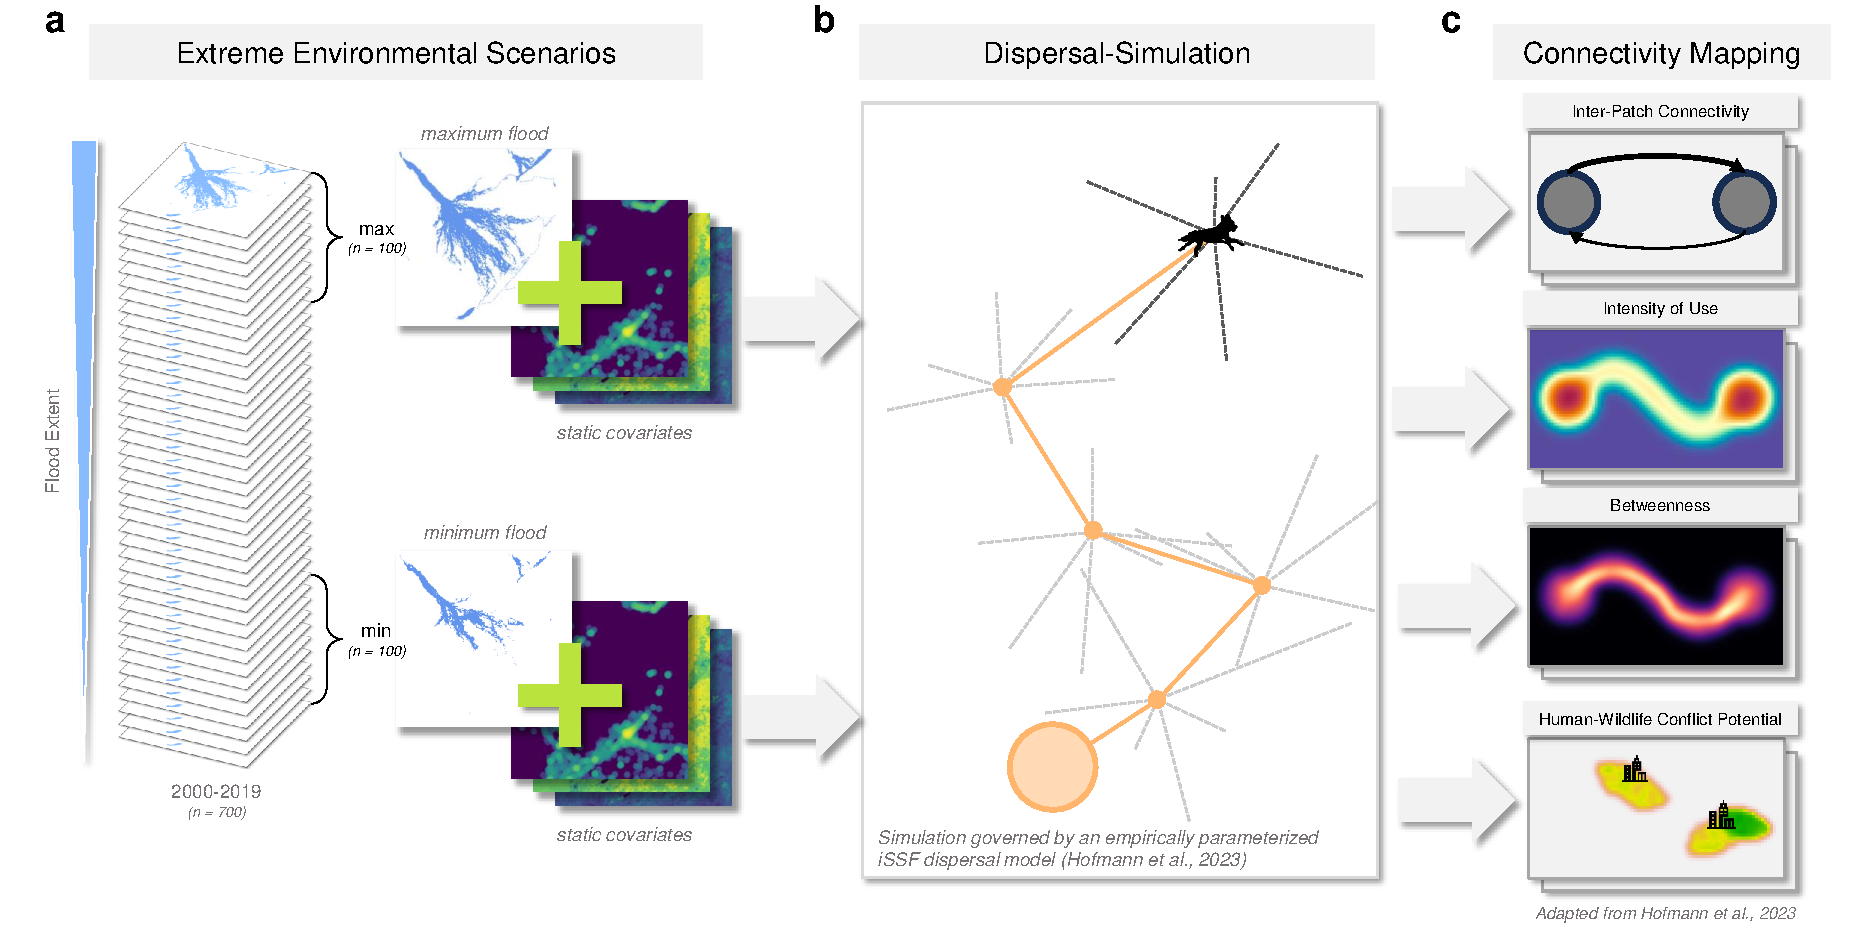
\includegraphics[width = \textwidth]{Figures/GraphicalAbstract.pdf}
  \caption{Conceptual illustration of the employed analytical framework to
  investigate connectivity for dispersing African wild dogs under a minimum and
  maximum flood extent in the Okavango Delta. (a) Based on a series of 700
  floodmaps, obtained between the years 2000 and 2019, we derived extreme
  scenarios for a minimum and maximum flood, using the minimum 100 and maximum
  100 historically observed flood extremes. These layers were then joined with a
  static set of covariates and fed into a dispersal simulation. (b) The
  dispersal simulation was based on a previously parametrized integrated
  step-selection function for dispersing wild dogs and allowed simulating
  dispersal trajectories in the two extreme scenarios. (c) From simulated
  dispersal trajectories we generated four summary maps, highlighting
  connectivity patterns and areas potentially prone to human-wildlife conflict.}
  \label{Concept}
 \end{center}
\end{figure}

\section{Materials and Methods}

\subsection{Study Area}

To investigate the effects of flood extremes on dispersal and connectivity, we
focused on a \textit{core study area} of 70,000 km\textsuperscript{2} that
comprised the Delta and its surroundings (\Cref{StudyAreaCH2}b; purple circle).
To accommodate for the long-distance dispersal events observed in this ecosystem
\citep{Cozzi.2020, Hofmann.2021, Cozzi.2023}, we also considered an
\textit{extended study area} of  300,000 km\textsuperscript{2} spanning from
21\degree 30' S to 17\degree 30' S to and 20\degree 30' E to 26\degree E and
comprising the Delta and parts of Angola, Namibia, Botswana, Zimbabwe, and
Zambia (\Cref{StudyAreaCH2}a). Rainfall in this area averages at 450 mm and is
mainly concentrated to the wet season between November and April
\citep{Mendelsohn.2004}. Even though local rains and ground table levels
resulting from floods of previous years may impact annual flood levels
\citep{McCarthy.2006}, the Delta's flood extent is primarily driven by
precipitation patterns in its catchment areas in the Angolan highlands, from
where water is channeled into the Cubango and Cuito rivers and subsequently
discharged into the Okavango Delta \citep{McCarthy.1997, McCarthy.2003}. Since
water only slowly descends from the catchment areas into the Delta and across
its shallow alluvial fan (gradient $\sim$ 1/3,400, \citealp{McCarthy.1997}), the
flood usually reaches its maximum extent long after the local rains have ceased,
during the peak dry season in July or August. Once the floodwater reaches the
Delta's distal ends, it percolates at the Thamalakane and Kunyere Faults, two
natural fault lines at which the water-flow is hindered (\Cref{StudyAreaCH2}b).
After reaching its maximum extent, water evaporates or percolates and the flood
steadily retracts over subsequent months. Such inner-annual dynamics are further
amplified or buffered by multi-annual cycles in precipitation patterns across
Angola \citep{Wolski.2012}. Due to the intricate interplay between precipitation
patterns in Angola, local ground-table levels, evapotranspiration, and
anthropogenic water abstractions, predictions of the flood extent under climate
change have proven challenging and range from ``much drier'' to ``much wetter''
depending on employed climate scenarios \citep{Kgathi.2006, Wolski.2008,
Hughes.2011, Wolski.2012, Moses.2018}. In the core study area, the vegetation is
dominated by mopane forest (\textit{Colophospermum mopane}), mixed woodland
acacia-dominated (\textit{Acacia spp.}), and grassland \citep{Mendelsohn.2010}.
Human influence is relatively low and mainly concentrated around small villages
at the western and southern periphery of the Delta. The largest urban center is
Maun, a spread-out settlement at the south-eastern tip of the Delta. Large
portions of the core study area are designated as national parks, game reserves,
or wildlife management areas. Some remaining sections of land are used for
cattle farming and suffer from moderate levels livestock depredation and
associated human-wildlife conflict \citep{Gusset.2009, McNutt.2017}. The core
study area and its extended surroundings are part of the world's largest
transboundary conservation initiative, the Kavango-Zambezi Transfrontier
Conservation Area (KAZA-TFCA, \Cref{StudyAreaCH2}a), which attempts to
re-establish connectivity among several core habitats. Previous studies have
indicated that this initiative has high potential for improving connectivity
among subpopulations of various species \citep{Brennan.2020, Lines.2021},
including African wild dogs \citep{Hofmann.2021}. However, a better
understanding of connectivity within this ecosystem under climate change is
lacking.

\begin{figure}[htpb]
 \begin{center}
  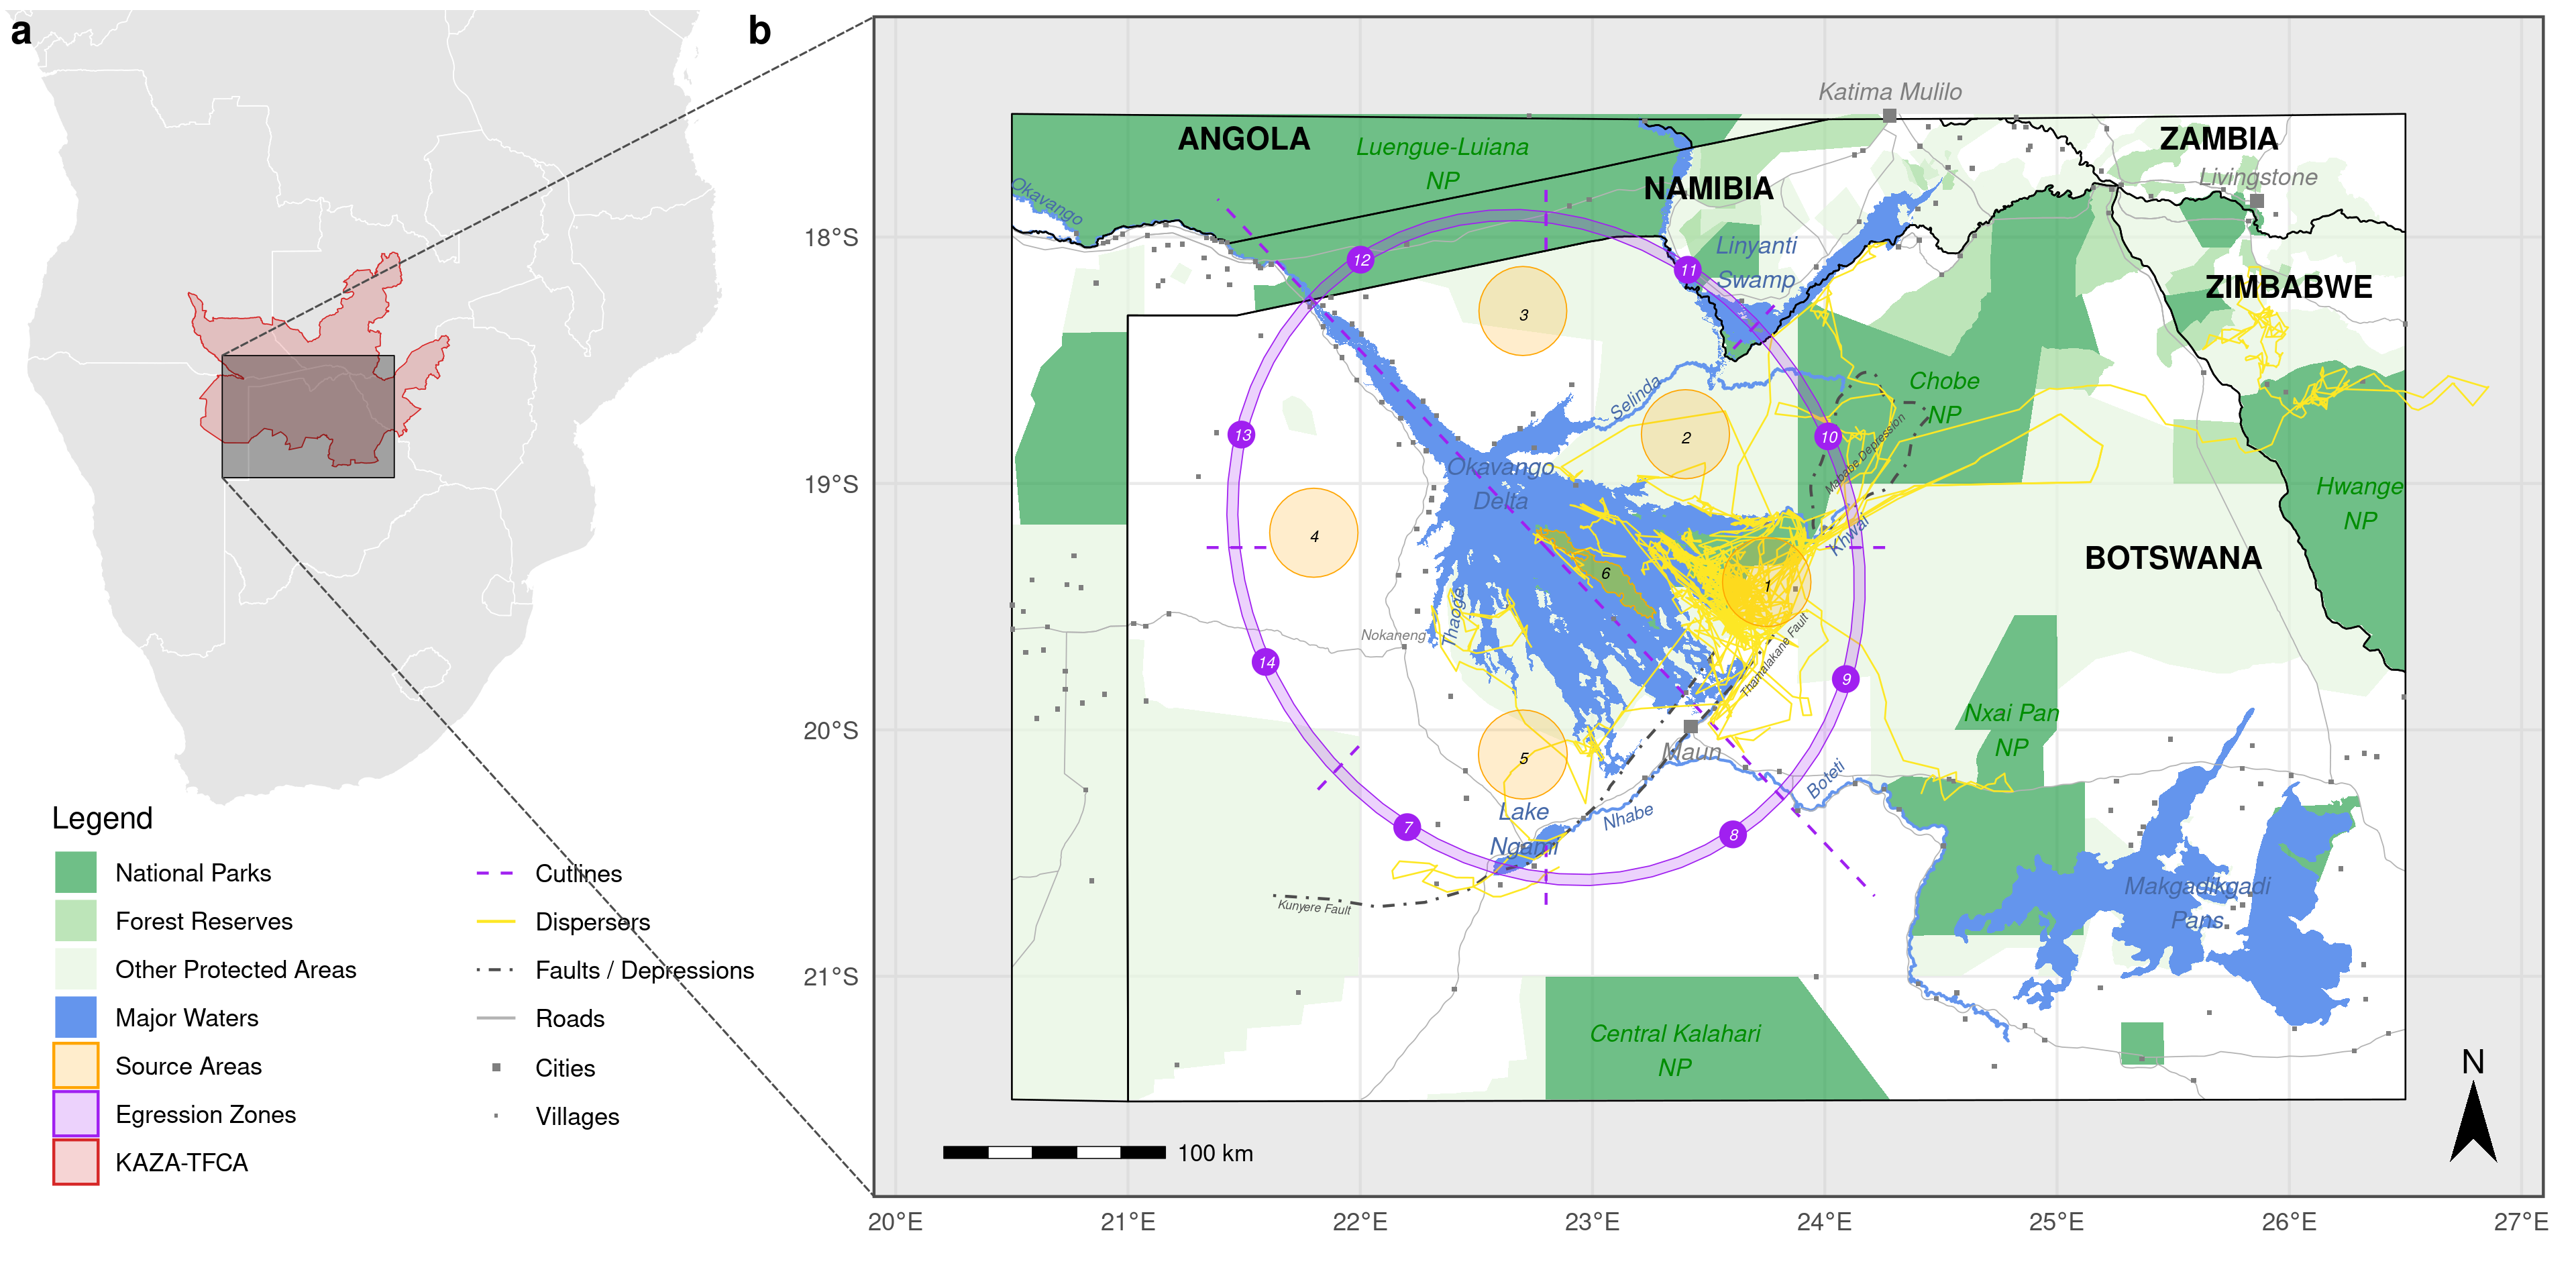
\includegraphics[width = \textwidth]{Figures/StudyArea2.png}
  \caption{(a) Location of the study area, which forms part of the
  Kavango-Zambezi Transfrontier Conservation Area (KAZA-TFCA, red polygon) in
  Southern Africa. (b) The division of the core study area (enclosed by the
  purple ellipse) into sub-areas (1 to 6) was based on the hydrographic
  structure of the Okavango Delta and its tributaries. We simulated dispersal
  trajectories starting at random locations within each of the six source areas
  (orange circles). Purple zones (7 to 14) represent zones that we used to
  identify if and where simulated dispersers left the close surroundings of the
  Okavango Delta (thus called egression zones). These zones were generated using
  a set of cutlines (purple dotted lines) originating from the center of the
  Delta that dissected an elliptical buffer surrounding the Delta into sections
  of equal size and in accordance with cardinal directions. The yellow lines
  represent GPS trajectories of dispersing wild dogs that were observed using
  GPS collars. While not all of these individuals were used to parametrize the
  dispersal model presented by \citet{Hofmann.2023}, they serve to highlight the
  spatial scale at which the species disperses.}
  \label{StudyAreaCH2}
 \end{center}
\end{figure}

\subsection{Spatial Habitat Layers}

We represented the physical landscape through which dispersers could move by a
set of spatially referenced habitat layers, each with a resolution of 250 m x
250 m. The set of layers included \textsf{water-cover, distance-to-water,
tree-cover, shrub/grassland-cover}, and a composite \textsf{human influence}
layer representing settlements, roads, and agricultural areas. A detailed
description of these layers is provided by \citet{Hofmann.2021}. However, unlike
Hofmann and colleagues, who used a single, static flood map, we employed
composite flood maps to study connectivity. Specifically, we generated
water-cover layers using MODIS Terra MCD43A4 satellite imagery that we
classified into binary water-cover maps using an algorithm developed by
\citet{Wolski.2017} and implemented in \texttt{R}
(\url{https://github.com/DavidDHofmann/floodmapr}). This algorithm allowed us to
generate weekly updated ``flood extent maps'', thus providing detailed
information about the flood at any given point in time. In total, we generated
700 flood extent maps, covering the years 2000 to 2019. We used these maps to
produce minimum and maximum flood scenarios, representative of dry and wet
climatic conditions, assuming that climate change will shift the system towards
one of these extremes in the long run. To create the baseline minimum (and
respectively, maximum) flood scenario, we averaged the 100 flood extent maps
with the smallest (highest) flood extent and generated a binary layer by masking
all pixels that were inundated in less than 50\% of the maps (see also
\Cref{Concept}). By averaging across 100 flood extent maps, we followed a
conservative approach and mitigated chances of misrepresenting minimum and
maximum flood extent due to inaccuracies or artifacts in single remote sensed
flood extent maps. The final minimum and maximum flood extent maps
(\Cref{FloodExtent}) show that the flood in the two scenarios covers
\inputy{Figures/FloodExtentMinimum.tex} km\textsuperscript{2} and
\inputy{Figures/FloodExtentMaximum.tex} km\textsuperscript{2}, respectively.
Finally, we combined the two flood extent maps with the set of above-mentioned
habitat layers into two spatial stacks, each representative of one scenario
(\Cref{Concept}). To prevent edge effects during the dispersal simulation, we
followed \citet{Koen.2010} and expanded the stacks to an extent that was 20\%
wider and taller than the original, filling the so created buffer zone (gray
buffer in \Cref{StudyAreaCH2}b) with randomized values from the respective
layers. This would allow simulated dispersers to leave and re-enter the main
study area via randomized buffer zones.

\begin{figure}[htpb]
 \begin{center}
  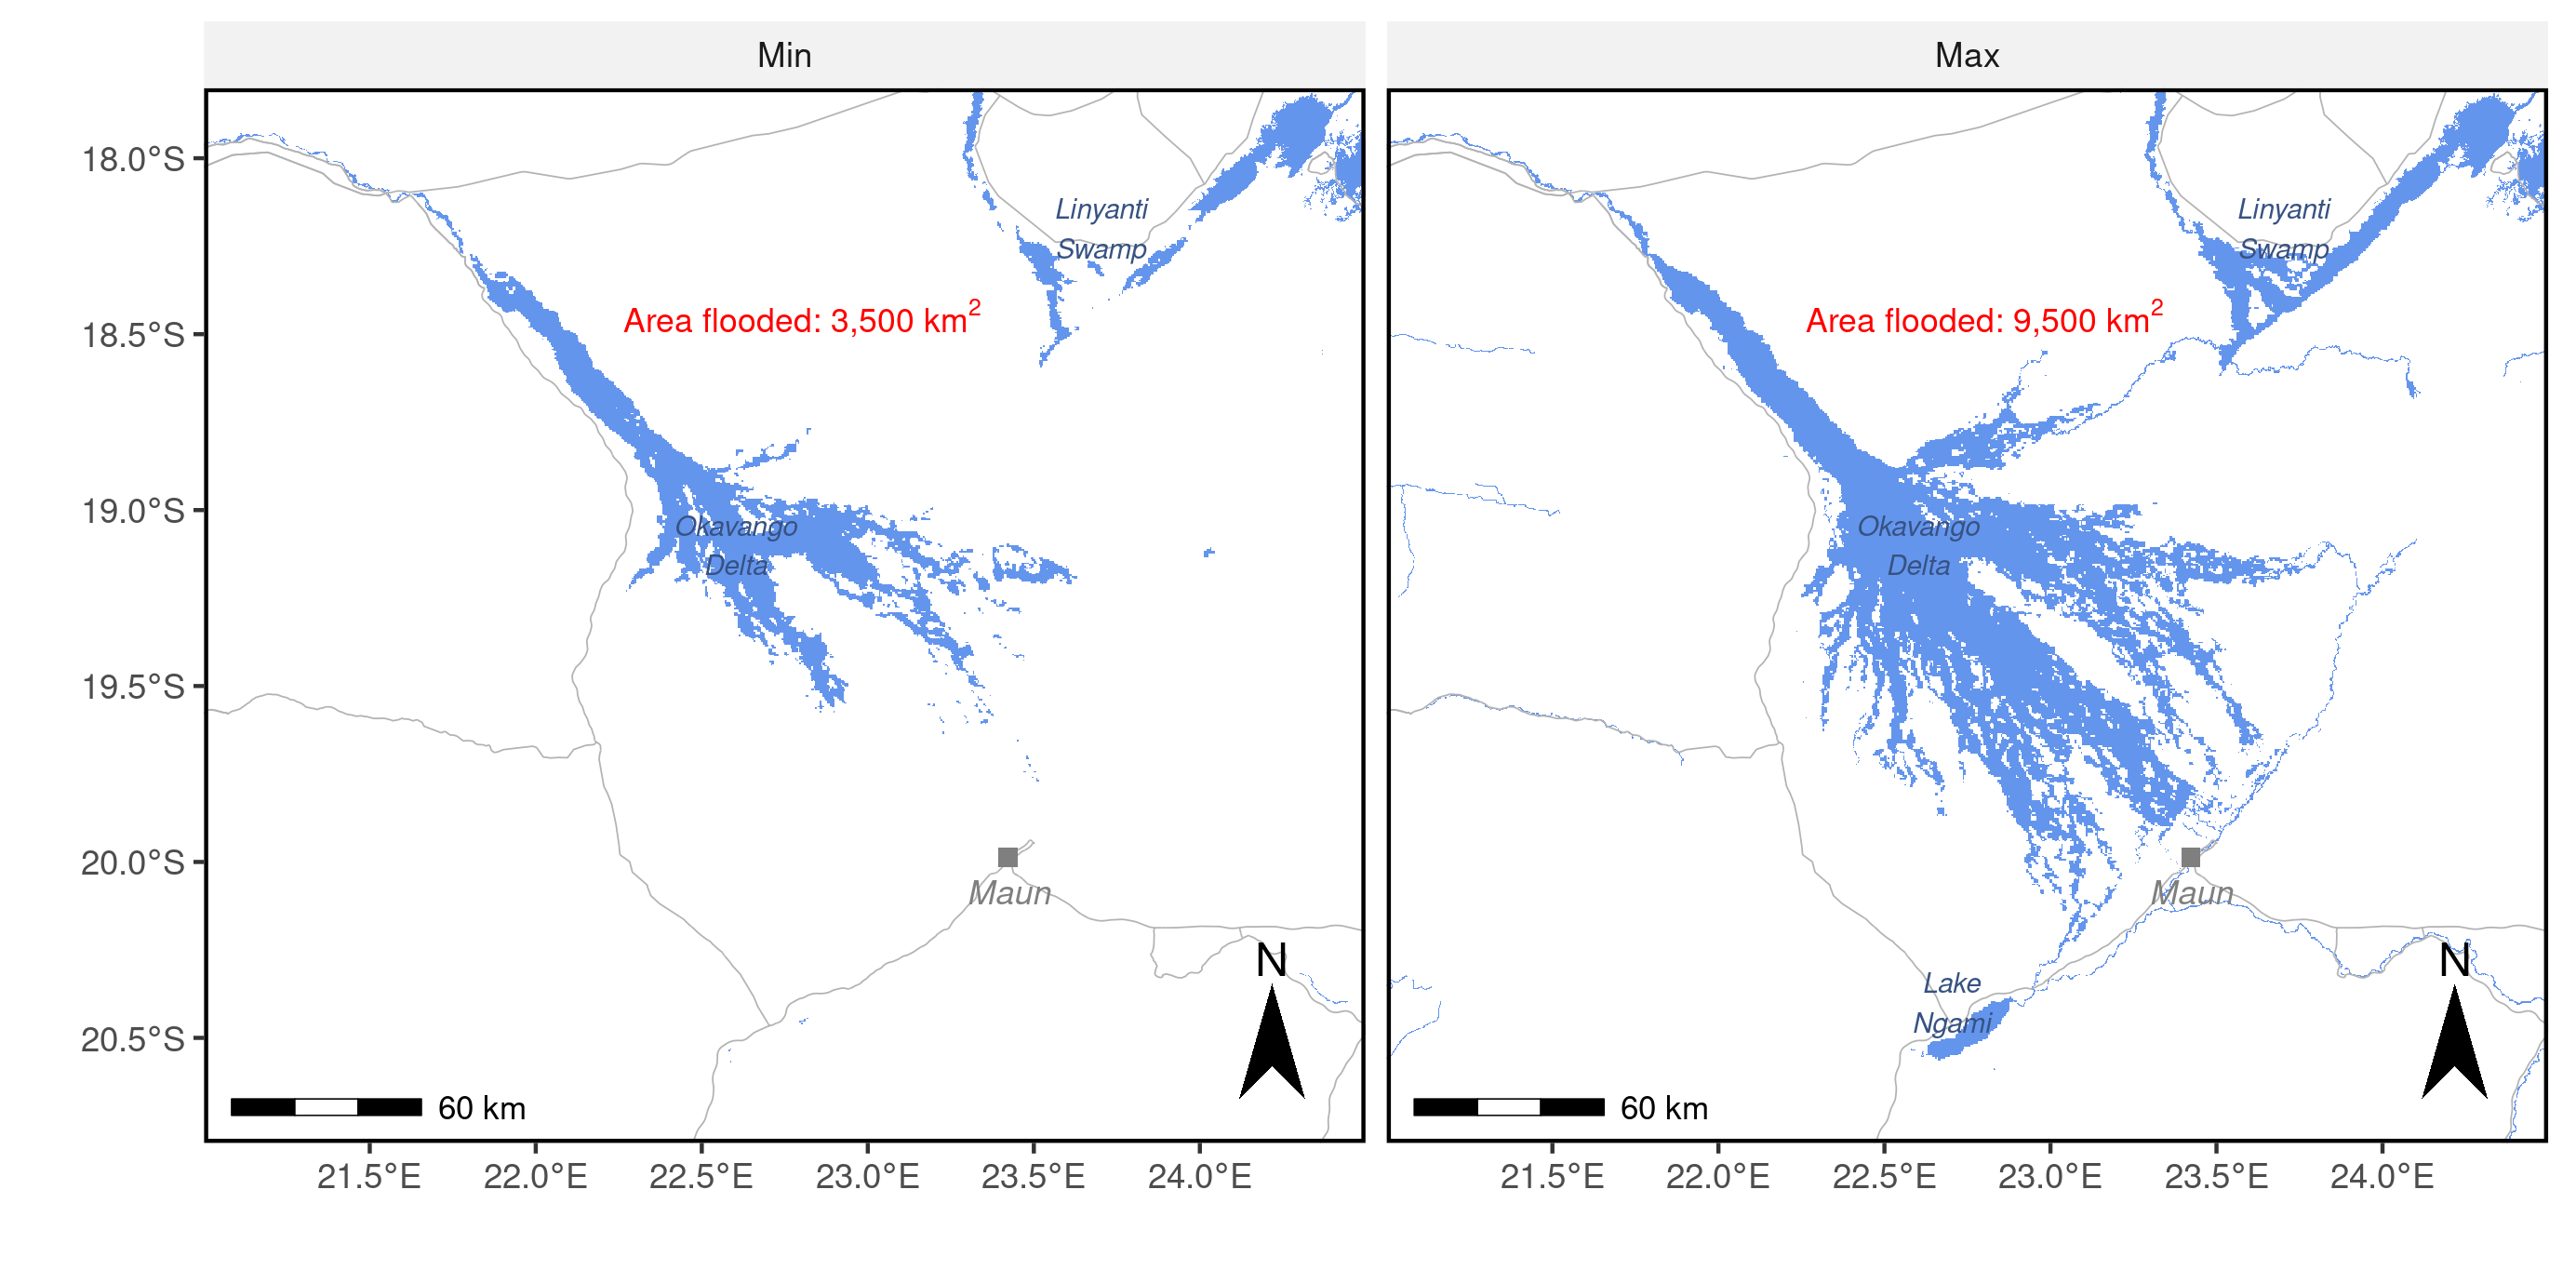
\includegraphics[width = \textwidth]{Figures/FloodExtent.png}
  \caption{(a) Minimum and (b) maximum flood extent. The two maps were generated
  based on 100 minimum and 100 maximum flood extent maps from a series of 700
  almost weekly updated remote sensed MODIS MCD43A4 satellite images spanning
  the years 2000 to 2019.}
  \label{FloodExtent}
 \end{center}
\end{figure}

\subsection{Source Areas and Egression Zones}

We simulated dispersing wild dogs originating from six distinct \textit{source
areas} located within the main study area (\Cref{StudyAreaCH2}b). Defining these
source areas was necessary to enable identification and quantification of the
number of successful dispersal events between different regions of the core
study area across the two flood scenarios. We selected source areas in regions
that remained dry during both scenarios and are known to host viable African
wild dog subpopulations. Nevertheless, these areas are not exhaustive and viable
wild dog populations are known to reside outside of them. The study area
comprises mostly of continuous habitat, yet natural and anthropogenic landscape
features allow the subdivision of the core study area into several sub-regions.
The Delta's hydrography and human settlements at its southern fringes result in
a natural latitudinal split between the eastern (areas 1, 2, and 3) and western
(areas 4 and 5) Delta (\Cref{StudyAreaCH2}b). Areas 1 and 2 are separated
longitudinally by the Selinda Spillway, a waterway that connects the Delta with
the Linyanti Swamp, while areas 2 and 3 are separated by the Khwai River, which
inundates the Mababe Depression east of the Delta (\Cref{StudyAreaCH2}b). On the
western side of the Delta, areas 4 and 5 are longitudinally separated by the
Thaoga River drainage at Nokaneng (\Cref{StudyAreaCH2}b). Finally, the Delta
hosts a central island, known as Chief's Island, which we defined as source area
6 (\Cref{StudyAreaCH2}b). The shape of this area was determined by its borders
towards water during the maximum flood scenario, whereas all other source areas
were defined using circular polygons with radii of 20 km at somewhat equal
distances to each other. We deliberately selected equally sized areas to
facilitate comparability between them and to minimize variability in simulated
connectivity due to target-effects. We also avoided source areas that directly
bordered each other, as simulated individuals initiated close to a shared border
would immediately result in connectivity and obscure differences between the two
scenarios. Besides source areas 1 to 6, we also generated \textit{egression
zones} (\Cref{StudyAreaCH2}b). These zones enabled us to determine through which
regions simulated individuals left the core study area, as well as to identify
after how many simulated steps they did so. We generated these zones by
overlaying the Delta with an ellipse that we dissected into equally sized
polygons in accordance with cardinal directions (\Cref{StudyAreaCH2}b). Overall,
the selection of source areas and egression zones was based on a mixture between
biological and computational considerations.

\subsection{Dispersal Simulation}

We used a previously parameterized and validated dispersal model to simulate
dispersal of African wild dogs. This dispersal model was trained using GPS data
obtained from 16 wild dog coalitions dispersing across northern Botswana
\citep{Hofmann.2023}. These data were collected at a sampling rate of four
hours, with the exception of one GPS location in the afternoon being skipped in
order to accommodate the species tendency to be less active during this period
(details in \citealp{Cozzi.2020, Hofmann.2021}). As such, a total of five GPS
locations were collected per day. The collected data were then fed into an
integrated step-selection function (iSSF, \citealp{Avgar.2016}), where
consecutive GPS locations were converted into \textit{observed steps} (the
straight-line connecting two consecutive GPS recordings; \citealp{Turchin.1998})
and compared to a set of \textit{random steps} using (mixed effects) conditional
logistic regression (\citealp{Fortin.2005, Thurfjell.2014, Muff.2020,
Fieberg.2021}; but see \citealp{Michelot.2024} for alternative approaches).
iSSFs provide less biased estimates of habitat-selection than traditional
resource-selection functions \citep{Forester.2009, Zeller.2016} and bear the
benefit that random steps are drawn from parametric step-length and
turning-angle distributions, such that a model parametrized using iSSFs
resembles a fully mechanistic model from which movement can be simulated
\citep{Signer.2017, Potts.2023, Signer.2024}. In contrast to graph-based
connectivity models (e.g., least-cost path analysis or circuit-theory),
simulations from iSSFs alleviate the need for resistance surfaces, which are
often subjective \citep{Simpkins.2017, Marrec.2020} and overestimate conductance
in difficult to reach habitat \citep{Signer.2017, Hofmann.2023}. The dispersal
model presented by \citet{Hofmann.2023} comprised a habitat-selection function
(describing habitat selection), a movement kernel (describing dispersers'
movement capacities), and potential interactions between the two. According to
the parametrized model, the main characteristics of wild dog dispersal movements
are avoidance of water, avoidance of areas influenced by humans, and a
preference for directional and fast movements. The associated model parameters
(provided in \Cref{Model}) can be used to predict probabilities of a step being
chosen among a set of random steps (details in \Cref{DispersalModel}), which
allows to simulate movements in discrete time.

Originating from each of the six source areas (\Cref{StudyAreaCH2}b), we
simulated 2,000 individual dispersing trajectories, each composed of 2,000
steps. Two thousand steps corresponded to a dispersal duration of $\sim$ 400
days, which marks the longest dispersal duration recorded in the study area
\citep{Cozzi.2020, Hofmann.2021}. By simulating 2,000 steps, we generated the
maximum amount of information possible and did not limit connectivity by
defining a dispersal cap. Note that we assumed that individuals would not
disperse for longer than 2,000 steps, but did not model settlement explicitly.
This is because only little is known about how dispersing wild dogs locate
potential mates and a suitable territory to settle. Olfactory cues at shared
scent-marking sites appear to play a crucial role, yet these are extremely
difficult to find and monitor \citep{Apps.2022, Claase.2022}. We simulated 1,000
trajectories under the minimum flood extent, the remaining 1,000 under the
maximum flood extent. Across the six source areas, this resulted in the
simulation of a total of 12,000 individual dispersal trajectories, which
sufficed to achieve convergence in relevant connectivity metrics
\citep{Hofmann.2023}. The simulation procedure was based on the algorithm
described by \citep{Signer.2017} and \citet{Hofmann.2023} and works as follows.
A random location within the source area is defined as the starting point.
Originating from the starting point, a set of 25 random steps is generated by
sampling step lengths ($sl$) from a gamma distribution fitted to observed steps
(shape = 0.37, scale = 6,316) and turning angles ($ta$) from a uniform
distribution ($-\pi, +\pi$). Along each random step, the underlying spatial
covariates are extracted, and relevant movement metrics computed ($log(sl)$ and
$cos(ta)$). \(\beta-\)estimates from the fitted dispersal model are then used to
predict the probability of each step being chosen, given the step's associated
covariates and movement metrics, as well as characteristics of all other
proposed steps. Among the 25 proposed steps, one is chosen at random based on
assigned probabilities. The procedure is then repeated until a total of 2,000
steps is simulated.

\subsection{Derived Metrics}

Based on simulated dispersal trajectories, we quantified connectivity,
identified the emergence of alternative dispersal corridors, and highlighted
areas with elevated potential for HWC. Our approach drew upon the set of
complementary connectivity metrics for individual-based movement models
discussed by \citet{Hofmann.2023}, and was expanded to include a map
highlighting areas with elevated HWC potential. The set of connectivity metrics
comprised \textit{inter-patch connectivity} metrics, summarizing dispersal
success and duration into distinct habitat patches, \textit{heatmaps}, depicting
areas of intense use by dispersers, and \textit{betweenness maps}, highlighting
dispersal corridors and bottlenecks. Finally, the \textit{HWC maps} served to
reveal areas where simulated dispersers moved into the vicinity of
human-dominated landscapes. To illustrate differences between metrics during
maximum and minimum flooding, we computed difference maps for the heatmaps,
betweenness maps, and HWC maps.

\subsubsection{Inter-Patch Connectivity}

To measure inter-patch connectivity, we tallied the number of trajectories
successfully moving from one source-area to another and computed the average
minimum dispersal duration (in number of steps) required to make those
connections. Dispersal between two areas was said to be successful whenever a
trajectory originating from one area intersected with the polygon of another
area. If a trajectory moved through multiple areas, a connection into each of
them from the original source was recorded. We also estimated the number of
individual trajectories that left the core study area and moved into one of the
egression zones. To quantify variability in our estimates, we generated
bootstrap samples by randomly drawing 1,000 simulated trajectories per source
area 1,000 times with replacement and computing 95\%-percentile intervals.

\subsubsection{Intensity of Use}

To quantify intensity of use of different areas, we generated heatmaps (also
known as \textit{utilization distributions} or \textit{flow-maps}) by
superimposing the study area with a grid with a spatial resolution of 1 km x 1
km and determining the number of simulated trajectories traversing each grid
cell. Such maps are essentially movement-restricted permeability surfaces, thus
highlighting areas of intense use \citep{Signer.2017, Potts.2023, Hofmann.2023}.
Heatmaps are relatively insensitive towards the chosen resolution and a 1 km x 1
km grid appeared to provide a good balance between detail and computational
feasibility.

\subsubsection{Betweenness}

To compute spatially mapped betweenness scores, we overlaid the study area with
a grid that had a resolution of 2.5 km x 2.5 km and computed the frequency at
which simulated individuals transitioned from one grid-cell to another. A
cell-transition was said to occur whenever a simulated step crossed from one
grid-cell across or into another. In case the same individual repeatedly
realized the same cell-transition, we only counted a single transition to avoid
overemphasizing regions where individuals moved in circles. This procedure
resulted in a weighted edge-list that we used to compute weighted betweenness
scores for each grid-cell, i.e. the importance of the respective grid-cell in
facilitating movement into adjacent areas \citep{Bastille-Rousseau.2018,
Bastille-Rousseau.2020}. We computed betweenness using the \texttt{igraph}
\texttt{R}-package \citep{Csardi.2006}. Calculations of betweenness scores are
computationally demanding and result in discrete and narrow dispersal corridors
\citep{Hofmann.2023}. A higher map resolution thus results in increased
computation time and narrower corridors. In our case, a grid size of 2.5 km x
2.5 km provided a sensible compromise between computational efficiency and
biological relevance of emerging corridors (see also the appendix of
\citealp{Hofmann.2023}).

\subsubsection{Human-Wildlife Conflict}

To pinpoint potential hotspots for HWC, we identified regions where simulated
trajectories moved into the vicinity of human-dominated landscapes. For this, we
isolated locations along simulated trajectories that ranged $\leq$ 500 meters to
the nearest grid-cell with human influence $>$ 0. Based on the so isolated
coordinates, we generated density maps highlighting likely hotspots for HWC.
While this approach of mapping potential HWC ignores human population density,
we also generated a compound metric by multiplying the generated heatmaps with a
continuous human-influence map (\Cref{AlternativeHWC}). Notably, not every
animal in the vicinity of human-dominated landscapes implies conflict, hence we
chose to use the term \textit{potential} hotspots for HWC. We prepared these
maps at a resolution of 1 km x 1 km.

\subsection{Software}

We conducted all data preparation and analyses using the programming language
\texttt{R} \citep{RCoreTeam.2023}. For any spatial data manipulation, we used
the \texttt{R}-packages \texttt{terra} \citep{Hijmans.2024} and
\texttt{spatstat} \citep{Baddeley.2015}. Several helper functions for the
dispersal simulation algorithm were written in \texttt{C++} and imported into
\texttt{R} using the \texttt{Rcpp} package \citep{Eddelbuettel.2011}. Network
analysis was achieved in \texttt{igraph} \citep{Csardi.2006} and figures were
generated using \texttt{ggplot2} \citep{Wickham.2024} and \texttt{ggnetwork}
\citep{Briatte.2024}. All \texttt{R}-scripts required to replicate our analyses
are provided through an online repository. Notably, a similar simulation
procedure as employed in our analysis has recently been added to the
\texttt{amt} \texttt{R}-package \citep{Signer.2024}.

\section{Results}
\subsection{Inter-Patch Connectivity}

Our analysis of inter-patch connectivity revealed significant differences in
dispersal success and duration depending on the flood scenario (\Cref{IPCTable},
\Cref{IPCMap}, \Cref{EmigrationImmigration}). Of the 6,000 simulated dispersal
trajectories for each flood scenario,
\inputy{Figures/NumberReachingOtherSourceAreasMinFlood.tex} trajectories reached
another source area during minimum flood, whereas
\inputy{Figures/NumberReachingOtherSourceAreasMaxFlood.tex} trajectories did so
during maximum flood, indicating a
\inputy{Figures/NumberReachingOtherSourceAreasMaxFloodPercent.tex}\% lower
dispersal success during maximum flood (\Cref{IPCTable}a1). Concurrently, the
average dispersal duration of trajectories moving from one source area to
another was
\inputy{Figures/DurationReachingOtherSourceAreasMaxFloodPercent.tex}\% lower
during maximum flood, with
\inputy{Figures/DurationReachingOtherSourceAreasMinFlood.tex} days compared to
\inputy{Figures/DurationReachingOtherSourceAreasMaxFlood.tex} days
(\Cref{IPCTable}b1) during minimum flood. The disparities were most pronounced
for trajectories dispersing into source area 6 (the Delta's center), with
\inputy{Figures/NumberReaching6MinFlood.tex} simulated trajectories reaching
area 6 during minimum flood compared to
\inputy{Figures/NumberReaching6MaxFlood.tex} trajectories (i.e.,
\inputy{Figures/NumberReaching6MaxFloodPercent.tex}\% lower) during maximum
flood (\Cref{IPCTable}a1). Source area 6 therefore appeared to be particularly
vulnerable to isolation in the maximum flood scenario. Interestingly,
connectivity between some source areas was higher during maximum flood. For
instance, the number of trajectories running from area 5 into area 4 was
\inputy{Figures/Connectivity5to4MaxFloodPercent.tex}\% higher, with
\inputy{Figures/Connectivity5to4MinFlood.tex} trajectories during minimum flood
compared to \inputy{Figures/Connectivity5to4MaxFlood.tex} trajectories during
maximum flood (\Cref{IPCTable}a1). Simulated individuals therefore responded to
unfavorable habitat conditions by dispersing into another region of the
landscape. Contrary to our expectations, movement into egression zones (areas 7
- 14) was only marginally higher during maximum flood, with the number of
trajectories rising by \inputy{Figures/EgressionMaxFloodPercent.tex}\%, from
\inputy{Figures/EgressionMinFlood.tex} to \inputy{Figures/EgressionMaxFlood.tex}
(\Cref{IPCTable}a2 and \Cref{Egression}).

\begin{table}
 \caption{(a) Dispersal frequency (measured as the number of dispersal
 trajectories) and (b) dispersal duration (in days) between (a1, b1) source
 areas (labeled 1 to 6) and (a2, b2) egression zones (labeled 7 to 14) during
 minimum and maximum flood. Final rows and columns of each subplot represent
 summary statistics across all areas. For instance, the bottom row in a1
 highlights for each source area the total number of trajectories successfully
 dispersing into a target area. The last column, in contrast, indicates the
 total number of trajectories immigrating into each target area. Values indicate
 mean $\pm$ SD. The colors are mapped in a non-linear fashion to avoid
 over-emphasis on final rows and columns.}
 \label{IPCTable}
 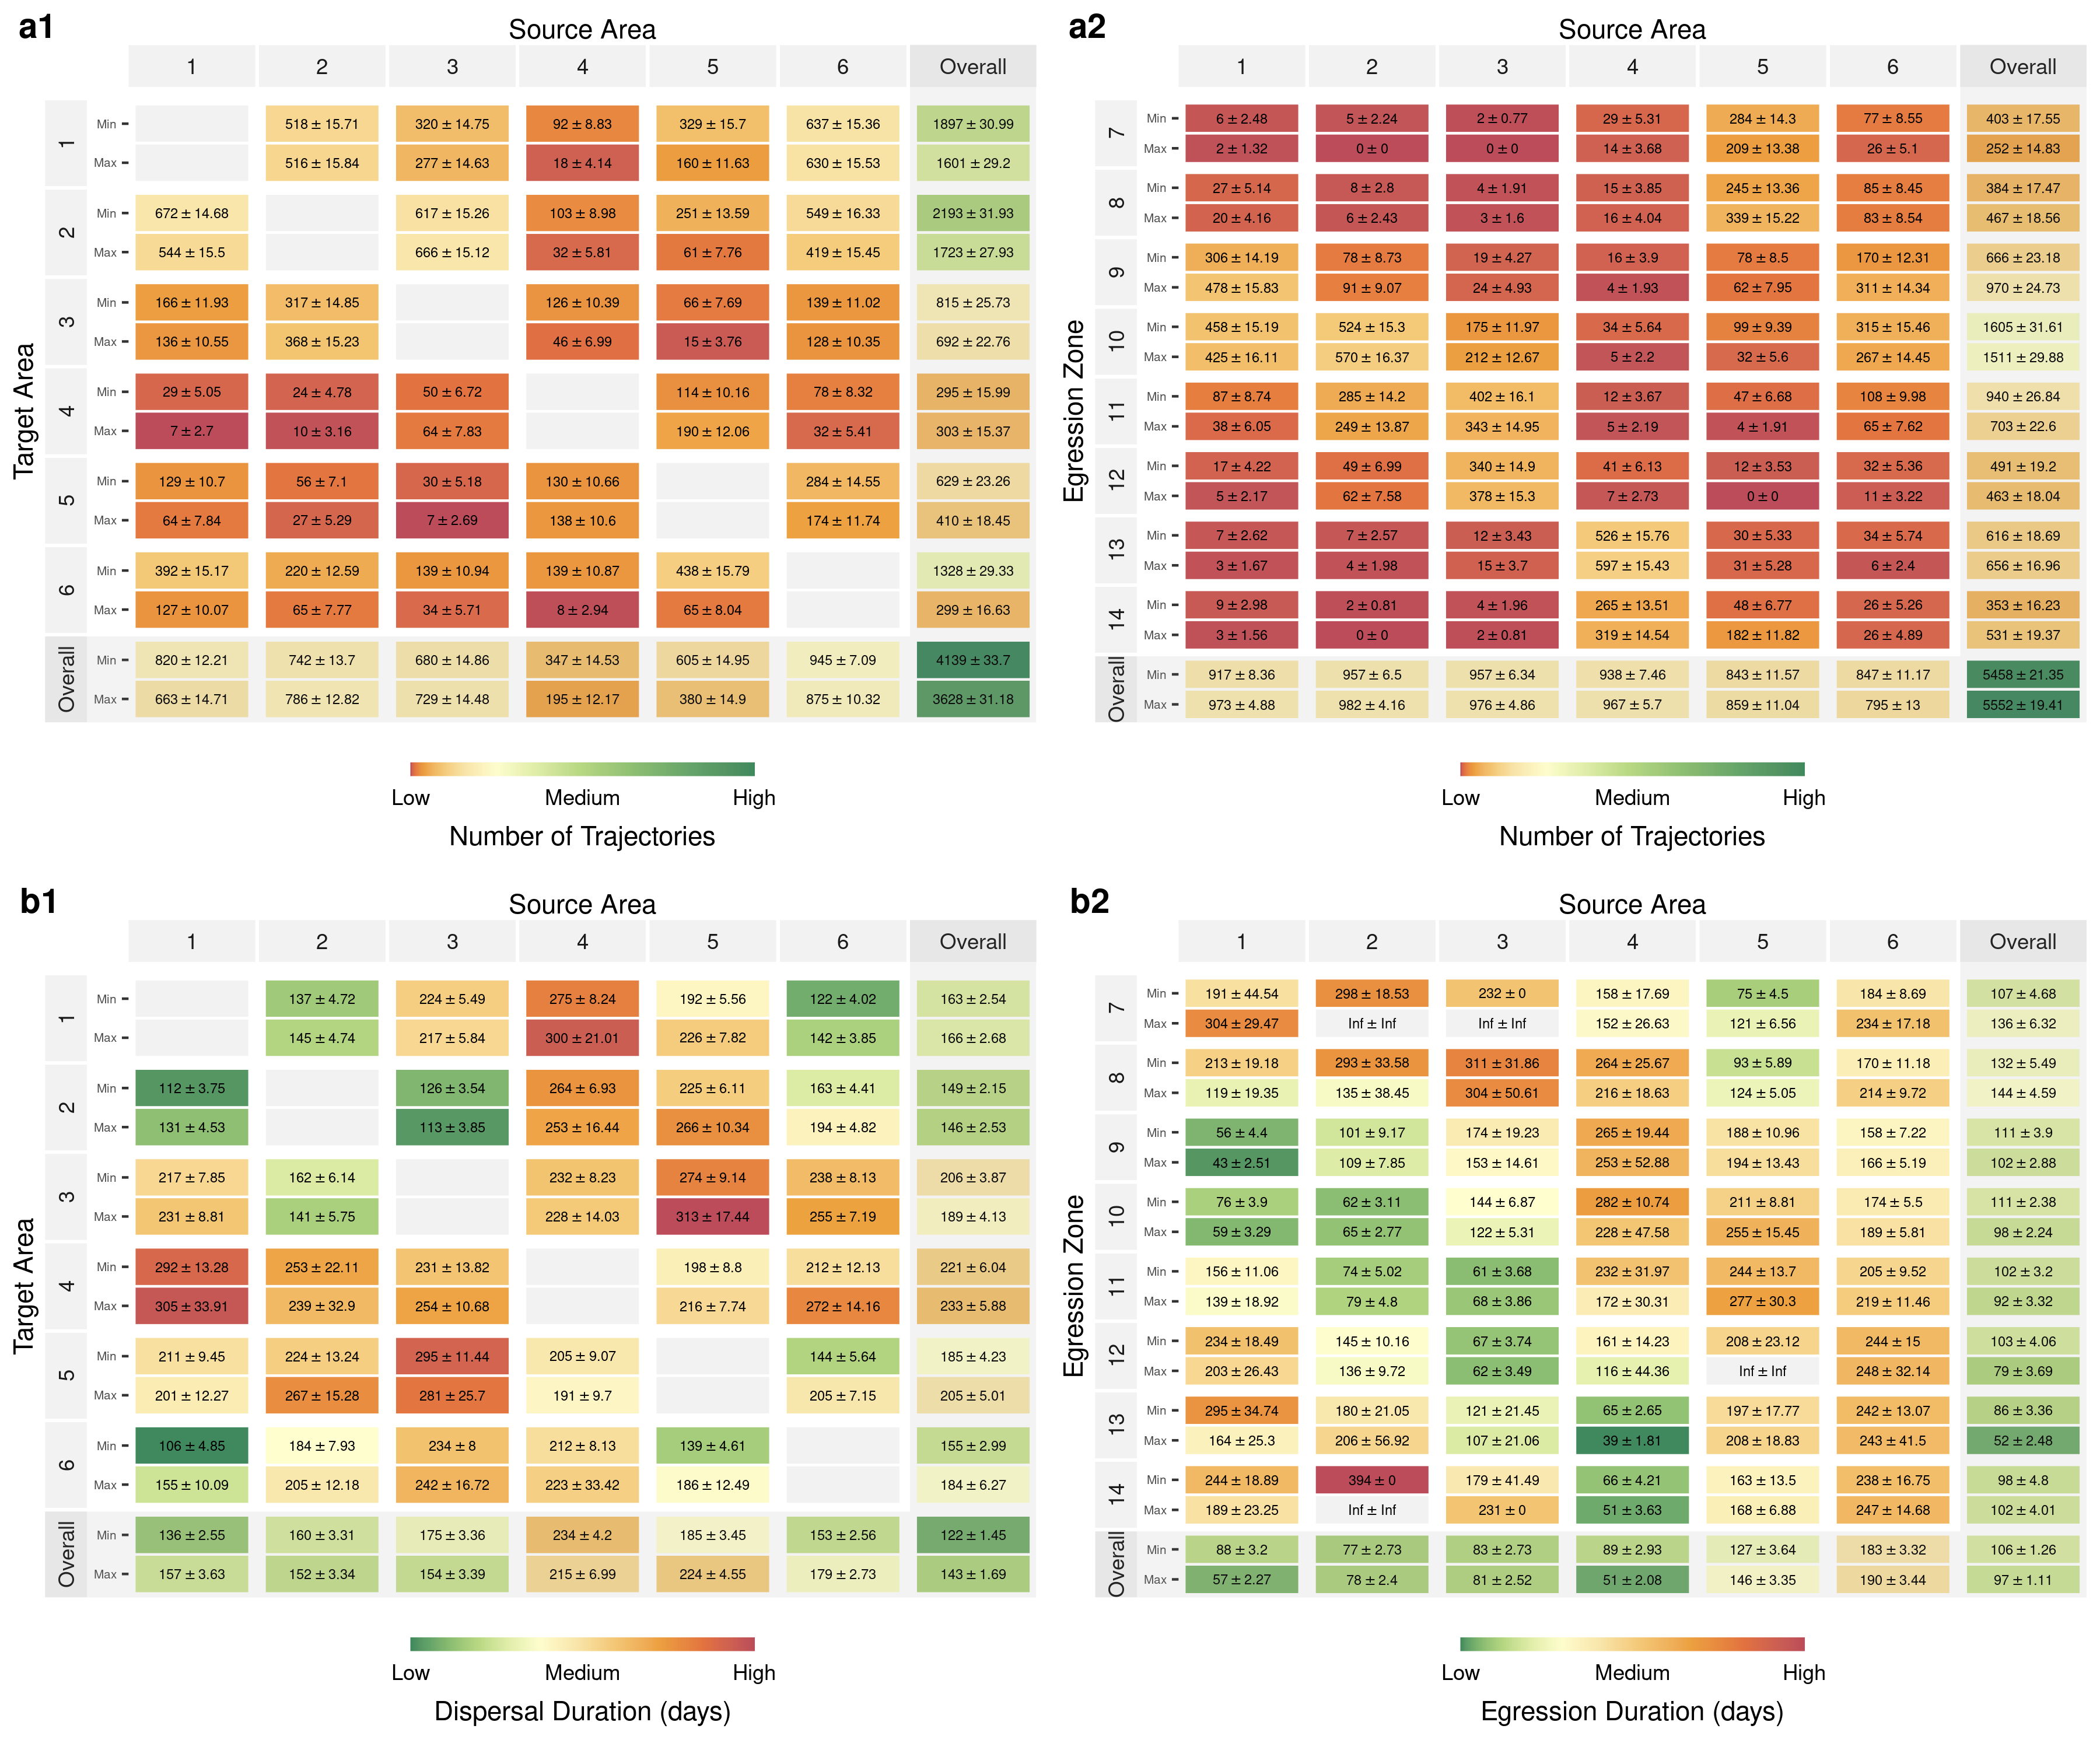
\includegraphics[width = \textwidth]{Figures/InterpatchConnectivityTable2.png}
\end{table}

\begin{figure}[htpb]
 \begin{center}
  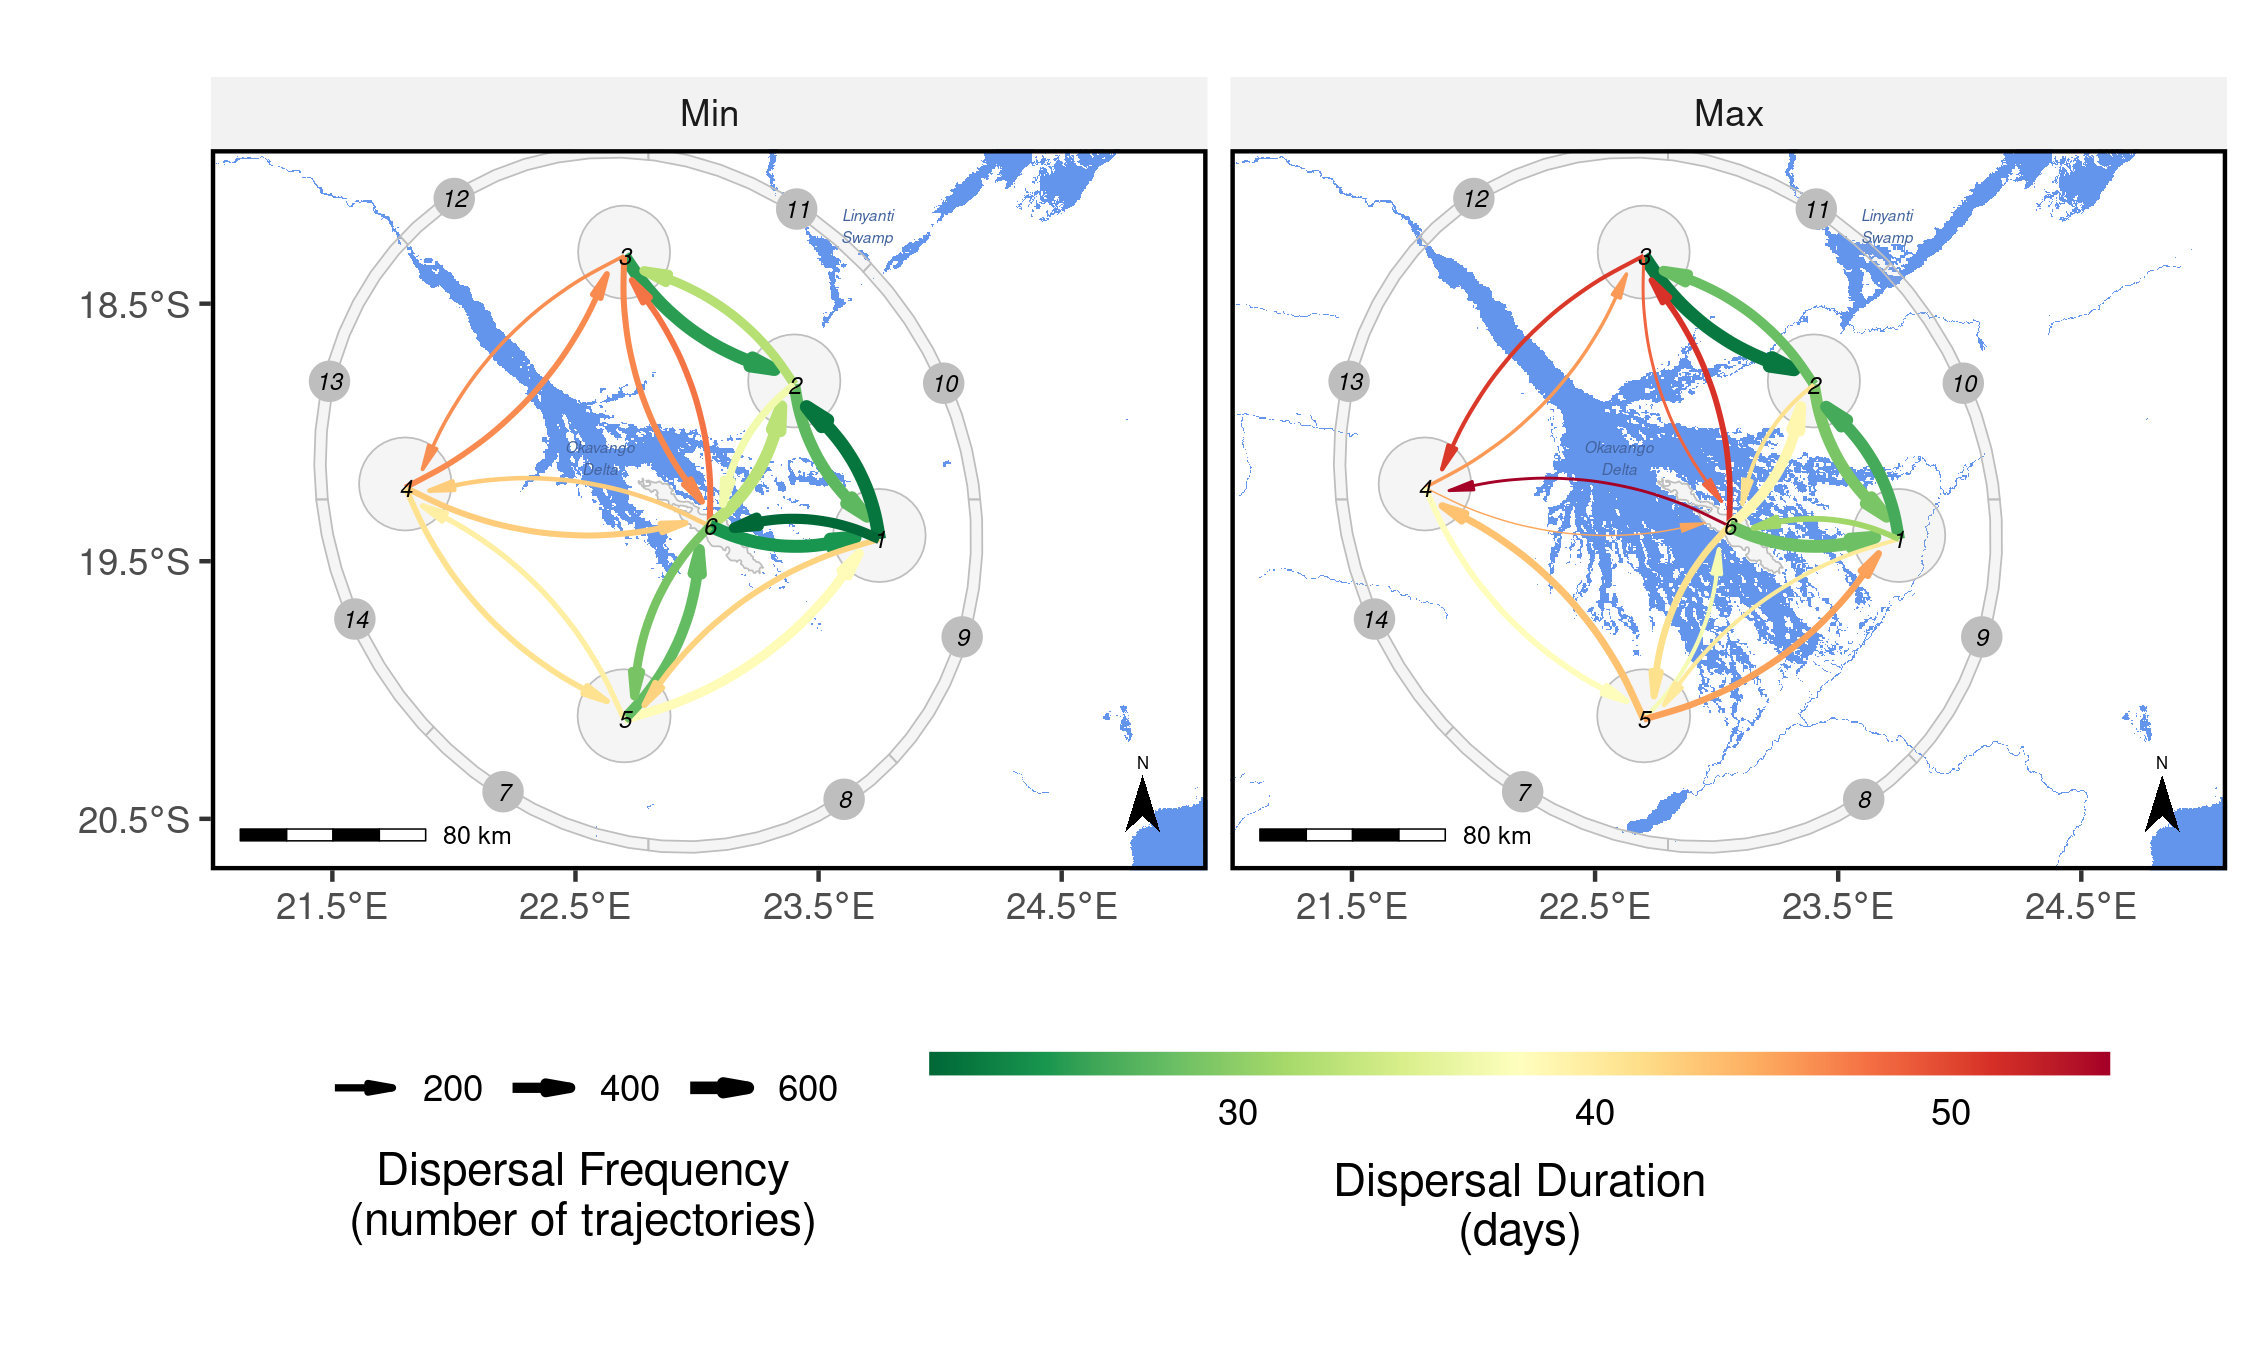
\includegraphics[width = \textwidth]{Figures/InterpatchConnectivityMap.png}
  \caption{Dispersal frequency and duration between source areas 1 to 6 in the
  core study area during the minimum (left panel) and maximum (right panel)
  flood scenario. The dispersal frequency shows the number of trajectories that
  emigrated from a specific source area and successfully immigrated into another
  one. The dispersal duration indicates the mean dispersal duration (in days)
  required before trajectories arrived at the respective area. Although links
  between non-neighboring source areas occurred in the simulation, we here only
  present links between adjacent source areas for brevity. Detailed plots about
  source-specific inter-patch connectivity are provided in \Cref{IPCMain} and
  \Cref{IPCBuffer}.}
  \label{IPCMap}
 \end{center}
\end{figure}

\subsection{Intensity of Use}

Heatmaps revealed that the Delta acted as a major dispersal barrier during
maximum flood, but became permeable during minimum flood (\Cref{Metrics}a).
During maximum flood, the floodwater extended from the Delta's inflow until the
densely inhabited regions at its southern fringes (the town of Maun and its
surroundings), such that the negative impacts of water on dispersal were further
aggravated by the negative effects of anthropogenic presence. Consequently,
there was a substantial decrease in the dispersal frequency across the southern
fringes of the Delta during maximum flood (\Cref{Metrics}a). During minimum
flood, however, the retracting flood revealed vast dispersal areas that
individuals used to move across the otherwise inundated regions
(\Cref{Metrics}a).

\subsection{Betweenness}

Findings from the betweenness maps, which display corridors and pinch-points
between neighboring areas, reinforced patterns observed on the heatmaps
(\Cref{Metrics}b). Multiple corridors linking source area 6 to the surrounding
source areas existed during minimum flood, but many of them vanished during
maximum flood (\Cref{Metrics}b). Instead, a single corridor at the south-eastern
tip of the Delta emerged (\Cref{Metrics}b). Despite the corridor's high
betweenness score, its apparent ability to link the eastern and western sections
of the Delta was limited, as evidenced by a low traversal frequency on the
heatmap (\Cref{Metrics}a).

\subsection{Human-Wildlife Conflict}

The HWC maps highlighted two potential hotspots for HWC that depended on
climatic extremes (\Cref{Metrics}c). The first hotspot was located at the
Delta's inflow between source areas 3 and 4 and was most prominent during
minimum flood. During maximum flood, by contrast, the density of simulated
locations in the vicinity of humans decreased by
\inputy{Figures/DensityHWCPanhandlePercentage.tex}\% in this area
(\Cref{Metrics}c and \Cref{HWCDifference}). Another hotspot, albeit visually
less distinct, covered the region at the distal end of the Delta, extending
across the town of Maun (\Cref{Metrics}c). This area was particularly relevant
during maximum flood, with a density that was
\inputy{Figures/DensityHWCMaunPercentage}\% higher than during minimum flood
(\Cref{Metrics}c and Figure S9). The diversion of individuals from one area to
another depending on flood conditions therefore drives the emergence of
potential hotspots for HWC.

\begin{figure}[htpb]
 \begin{center}
  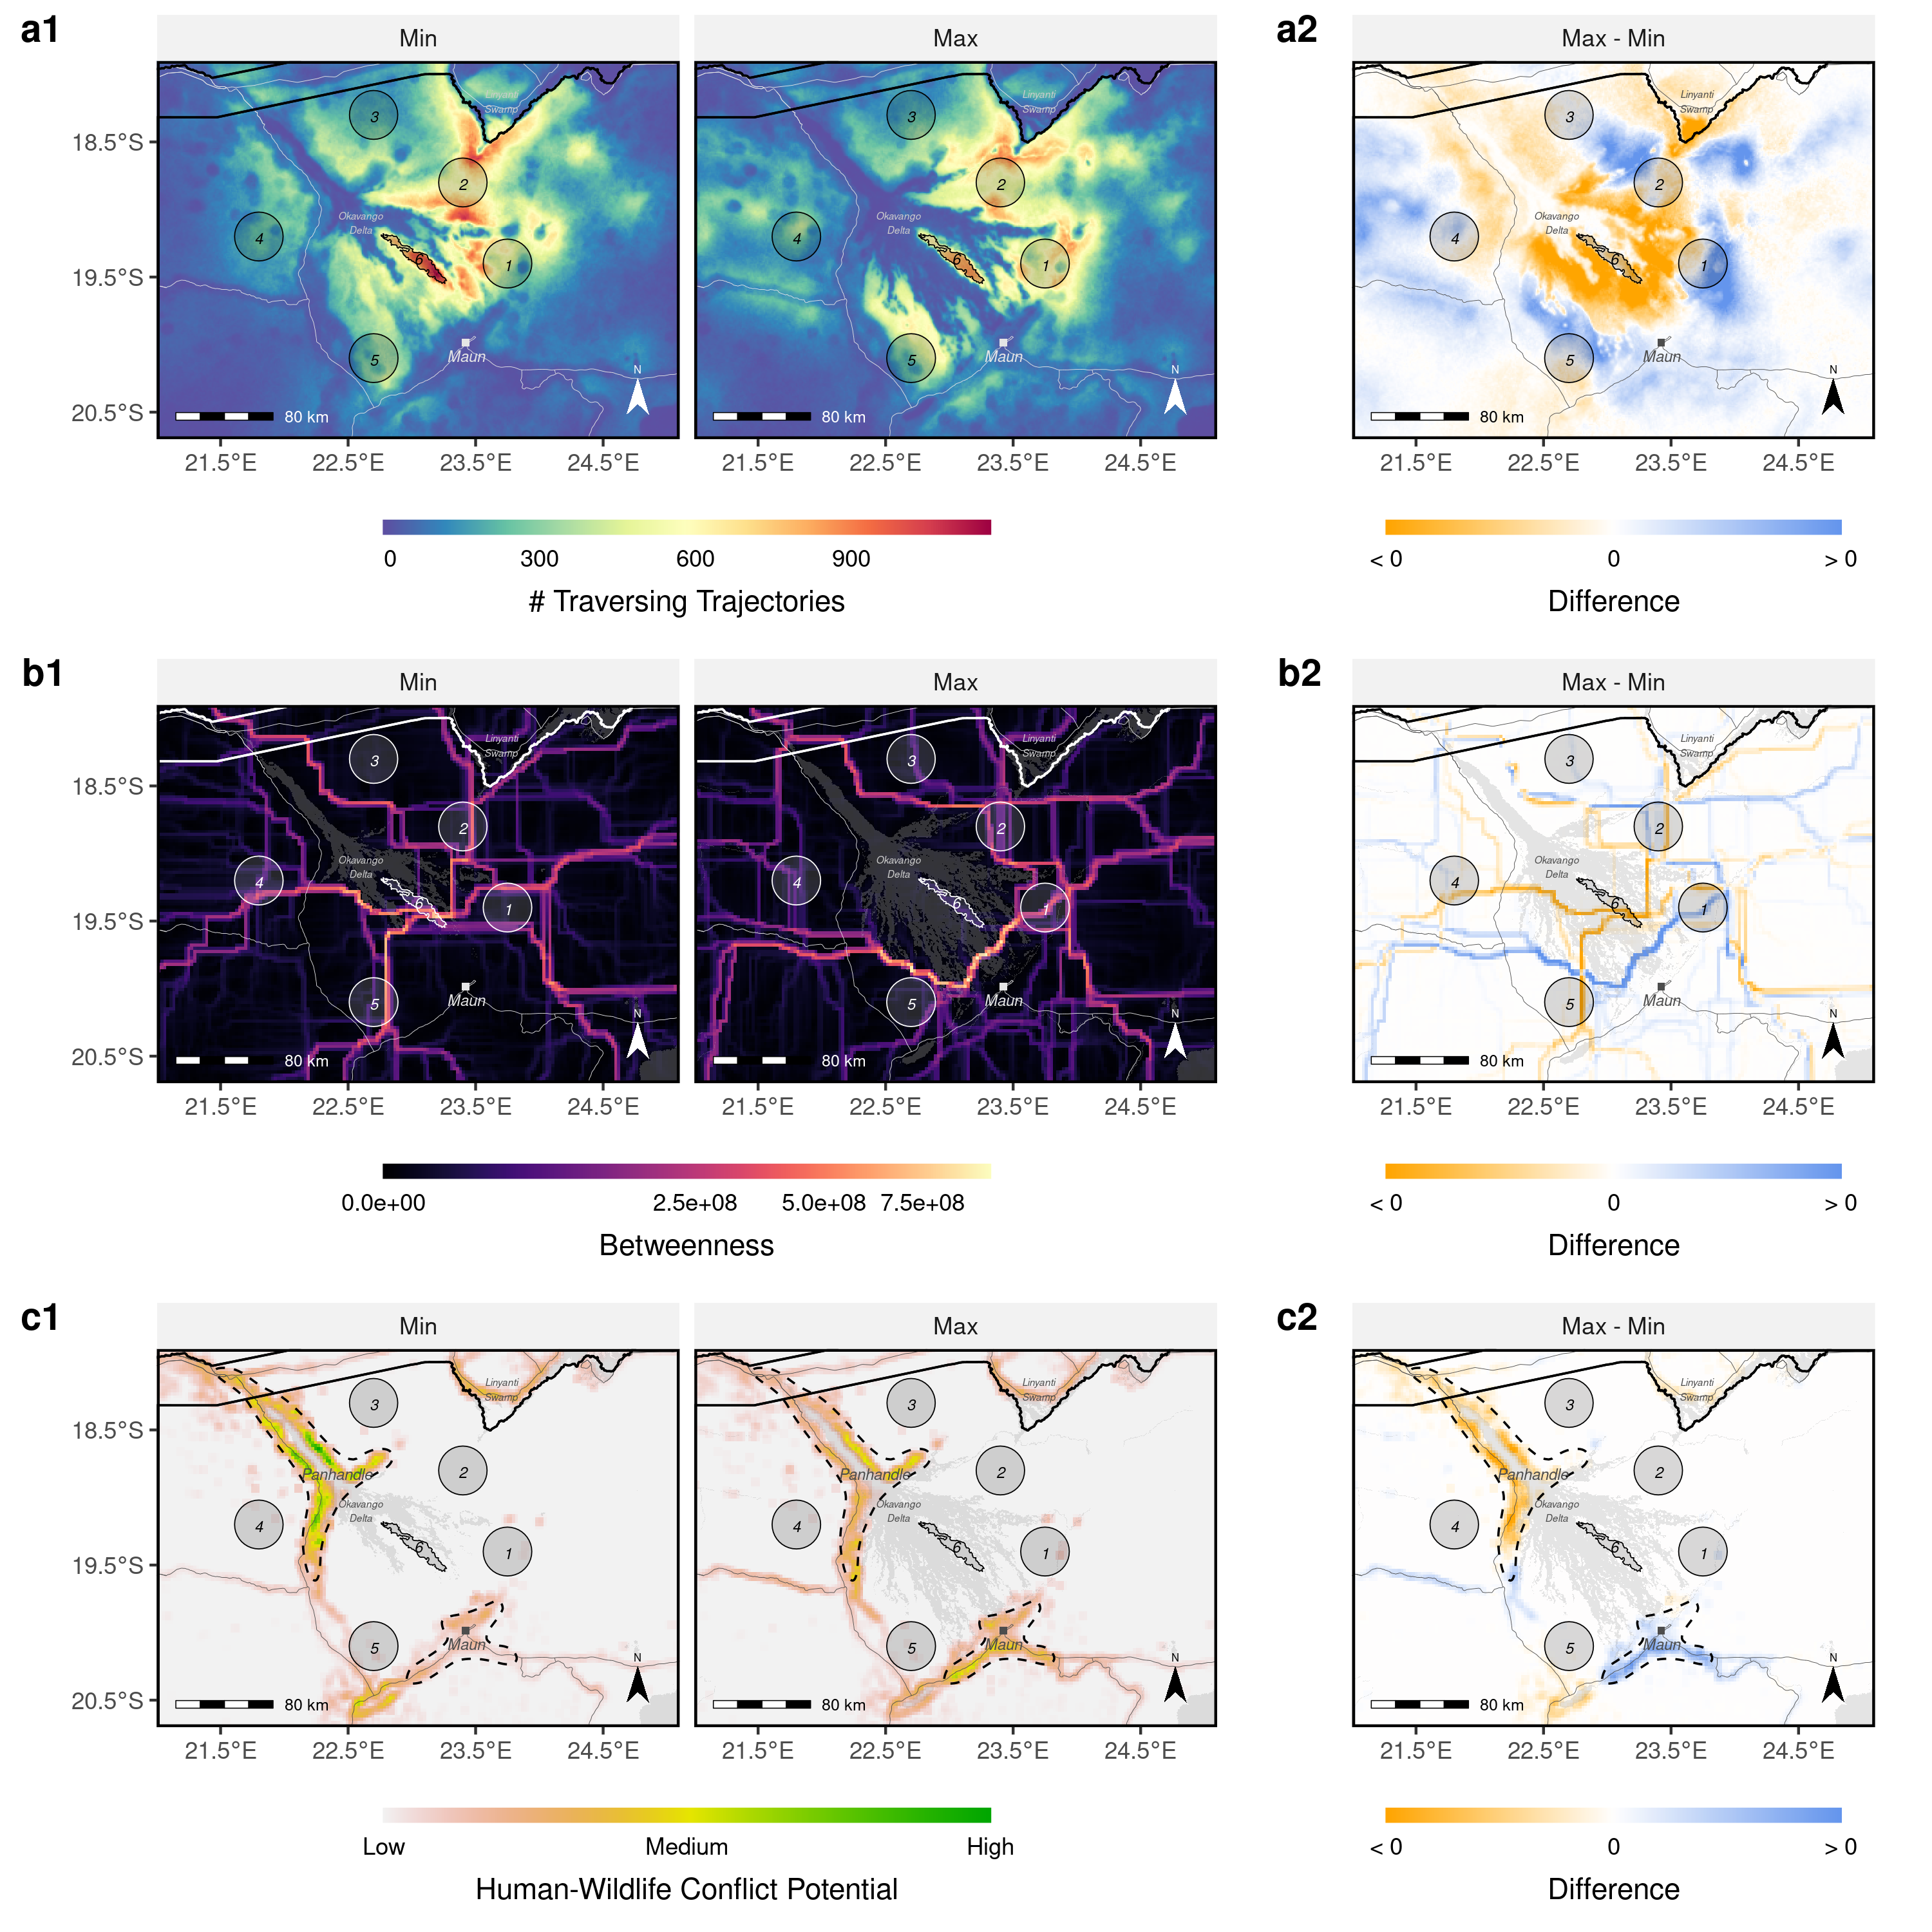
\includegraphics[width = \textwidth]{Figures/Metrics.png}
  \caption{(a) Heatmaps, (b) betweenness maps, and (c) maps of potential for HWC
  derived from simulated dispersal trajectories. Left panels were derived from
  the minimum flood scenario, right panels from the maximum flood scenario.
  Source areas from which dispersers were released are numbered 1-6. The color
  scale for betweenness scores in subfigure b was square-rooted to improve
  visibility of corridors with lower values. Source-specific heatmaps,
  betweenness maps, and HWC maps are provided in Figures \Cref{HeatmapsInd},
  \Cref{BetweennessInd}, and \Cref{HWCInd}.}
  \label{Metrics}
 \end{center}
\end{figure}

\section{Discussion}

% \subsection{Impacts of Extreme Environmental Conditions on Dispersal}

We investigated the impacts of extreme environmental conditions, as anticipated
under the influence of climate change, on dispersal and connectivity. For this,
we employed a previously parameterized and validated movement model and
simulated dispersal trajectories of African wild dogs in the Okavango Delta
under extreme conditions. Our findings indicate that an amplified flood can
significantly reduce dispersal success, prolong dispersal durations, and alter
the spatial structure of major dispersal corridors, thereby creating or
shifting hotspots of potential human-wildlife conflict (HWC).

Wetter-than-usual climatic conditions, a likely scenario for this study area
\citep{Wolski.2008, IPCC.2022}, resulted in significant barriers to dispersal
and connectivity, and in an overall increase in dispersal durations. This was
largely a result of simulated individuals avoiding large water bodies, thus
detouring through more suitable habitats \citep{Cozzi.2013, Cozzi.2020,
Hofmann.2021, Hofmann.2023}. Movement constraints due to changes in
environmental conditions can thus lead to subpopulation isolation (up to $>$
75\% in our case), thereby jeopardizing recolonization efforts following local
extinctions, and impacting population dynamics, gene flow, and genetic
diversity \citep{Hanski.1999, Frankham.2002, Leigh.2012, Baguette.2013}.

The African wild dog exhibits a remarkable dispersal ability, sometimes
dispersing several hundred kilometers across international borders
\citep{McNutt.1996, Davies-Mostert.2012, Masenga.2016, Cozzi.2020,
Sandoval-Seres.2022, Cozzi.2023}. This ability likely evolved as an adaptation
to the relatively low density at which the species occurs \citep{Creel.2002,
Masenga.2016} and may have been sustained by a historically well-connected
landscape that imposed low mortality (sensu \citealp{Fahrig.2007}). Today,
however, the need for vast dispersal habitats makes this species vulnerable to
habitat loss and fragmentation \citep{Woodroffe.2012, Woodroffe.2020}. When
dispersing animals are forced to alter their dispersal routes due to changing
environmental conditions, this could result in non-optimal dispersal behavior in
human-altered landscapes \citep{Fahrig.2007}. This is particularly problematic
when dispersers are channeled through areas with high anthropogenic resistance
and elevated risk of mortality \citep{Fahrig.2007, Ghoddousi.2021,
VanDerMeer.2014}. For a population of African wild dogs in Zambia,
\citet{Leigh.2012} revealed that dispersal and the associated mortality indeed
led to a decline in genetic diversity and, subsequently, to a net-loss of
individuals. At present, our own study population appears to benefit from
moderate levels of dispersal, as an analysis across Southern Africa revealed a
genetically healthy cluster in the Kavango-Zambezi Transfrontier Conservation
Area \citep{Tensen.2022}. This cluster may, however, be at risk depending on
future flood conditions.

% The redirection of dispersal paths coupled with altered climatic conditions and
% increased encroachment by humans, could therefore result in non-optimal
% dispersal behavior (sensu \citealp{Fahrig.2007}), especially when dispersers are
% forced to move across regions with high anthropogenic resistance and elevated
% risk of mortality \citep{Fahrig.2007, Ghoddousi.2021, VanDerMeer.2014}. Indeed,
% \citet{Leigh.2012} revealed that dispersal and the associated mortality led to a
% decline in genetic diversity in a population of wild dogs in Zambia and,
% subsequently, to a net-loss of individuals. At present, our study population
% appears to benefit from moderate levels of dispersal, as an analysis across
% Southern Africa revealed a genetically healthy cluster in the Kavango-Zambezi
% Transfrontier Conservation Area \citep{Tensen.2022}. This cluster may, however,
% be at risk depending on future flood conditions.

As dispersal is a key process influencing population dynamics
\citep{Hanski.1999, Clobert.2012}, any climatic-induced alteration will have
cascading effects that amplify or buffer the effect of climatic changes on
population persistence and viability. Lower connectivity and prolonged
dispersal durations due to adverse environmental conditions will inevitably
result in increased energetic expenditures and exposure to various threats such
as predation, competition, human encounters, and diseases \citep{Alberts.1995,
Yoder.2004, Stamps.2005, Bonte.2012}, thus further jeopardizing dispersal
success and its effect on population dynamics. Higher ambient temperatures have
previously been associated with negative effects on wild dog reproductive
success \citep{Woodroffe.2017, Abrahms.2022}, survival \citep{Rabaiotti.2021},
and, consequently, population persistence \citep{Rabaiotti.2023}. The negative
effect of hotter climatic conditions on local population survival and
recruitment may be further exacerbated by reduced dispersal success and
connectivity in case of amplified flooding regimes.

Even though our finding that an increased flood extent reduces connectivity
seems unsurprising, it is non-trivial to quantify such impacts and to predict
the spatial rearrangements of movement corridors they entail. Wild dogs avoid
crossing water bodies, yet are capable of doing so if they really need to,
especially during dispersal \citep{McNutt.1996, Cozzi.2013, Cozzi.2020,
Hofmann.2023}. By simply assuming such obstacles to be impenetrable, one may
miss important corridors that lead across narrow sections of unsuitable habitat
\citep{Marrec.2020}. Using simulations from integrated step-selection functions
(iSSFs), however, one can realistically render that an animals' decision to
disperse across a specific habitat is conditional on what's available at
alternative steps. A disperser surrounded by a hostile matrix may readily cross
water, whereas an individual dispersing through favorable habitat can choose to
avoid water entirely. Another challenge when predicting the impacts of climate
change on connectivity is that future on-the-ground conditions are rarely known
(e.g., \citealp{Wolski.2008}). To overcome this, we leveraged historic data on
seasonal variation of the flood extent and assumed that climate change would
shift the ecosystem towards conditions that currently mark extremes. A similar
approach can be applied in systems where the relationships between changing
conditions and functional connectivity are less evident.

While wet extremes appear to hinder dispersal and connectivity, the opposite
applies for amplified dry conditions, because areas that are inundated under
normal circumstances become free of water and therefore passable. Predictions
suggest that climate change will result in elevated precipitation across the
Delta's catchment areas in Angola \citep{Wolski.2008, IPCC.2022}, thus resulting
in above-average flooded regions. Concomitantly, however, hotter temperatures
and increased levels of evapotranspiration are anticipated for the Delta's basin
in Botswana, suggesting that dry periods may be experienced too
\citep{Wolski.2008, Moses.2018, Akinyemi.2019, IPCC.2022}. The Delta's expanse
is also affected by multi-decadal oscillations in precipitation patterns, which
may periodically offset or amplify long-term trends \citep{Wolski.2012}. The
overall impact of climate change on flood patterns therefore remains unknown
\citep{Wolski.2008, Wolski.2012} and this lack of knowledge is aggravated by
uncertainties regarding future anthropogenic water abstractions along the
Okavango River \citep{Kgathi.2006, Murray-Hudson.2006, Hughes.2011}. It is
nonetheless worth noting that our maximum flood extent map, which was prepared
based on 100 maximum flood extents observed on over 700 weekly-updated
floodmaps, is conservative compared to historically observed flood extents in
the Delta. While the flood in our map encompasses an area of
\inputy{Figures/FloodExtentMaximum.tex} km\textsuperscript{2}, the Delta may
inundate an area of up to 14,000 km\textsuperscript{2} in exceptional cases
\citep{McCarthy.2003, Gumbricht.2004}. Changes in dispersal behavior and
connectivity due to climate change may therefore be more pronounced than
reported here.

% \subsection{Human-Wildlife Conflict}

Our analysis revealed that dispersers utilize different movement corridors
depending on flood conditions, leading to the emergence and shifting of
potential hotspots for HWC. An increased proximity between humans and carnivores
is typically associated with a higher potential for conflict (e.g.,
\citealp{Michalski.2006, Chapman.2016}). Especially dispersers, which often
venture outside protected areas, expose themselves to anthropogenic hostility
\citep{Elliot.2014, Cozzi.2020, Vasudev.2023}. In our case, the funneling of
individuals through alternative dispersal corridors resulted in the shift of
potential HWC hotspots, potentially increasing HWC and retaliatory killing. One
example is the area surrounding Maun, where HWC is expected to rise during wet
periods, exacerbating existing human-wildlife conflict \citep{Gusset.2009,
McNutt.2017, Cozzi.2020}. Identifying and mapping the conflict-connectivity
interface (i.e., areas prone to HWC) in light of climate change can improve our
understanding of connectivity \citep{Vasudev.2023} and could aid in prioritizing
mitigation and prevention measures that have the highest impact
\citep{Treves.2011, Buchholtz.2020} or to develop appropriate compensation
schemes \citep{McNutt.2017}. However, it is important to note that encounters
between animals and humans do not imperatively imply HWC, and that the severity
of conflict and its impact on connectivity likely depends on humans' perception
and attitude towards wildlife \citep{Ghoddousi.2021}. Besides the risks
associated with direct mortality through human persecution, a higher proximity
to humans also increases the risk of indirect mortality through disease
transmissions from domestic animals \citep{Cleaveland.2000, VanDeBildt.2002}.
Previous outbreaks of distemper and rabies have caused the local extermination
of African wild dogs in several African countries \citep{Woodroffe.2004}. As
infected dispersing individuals may further spread diseases within protected
areas, a better understanding of points of interaction between humans and
wildlife will facilitate the implementation of targeted vaccination programs in
the face of climatic change \citep{Vial.2006}.

% \subsection{Methodological Limitations and Future Research Directions}

In the present study, we ignored mortality during dispersal and assumed all
simulated dispersers to survive for 2,000 steps ($\sim$ 400 days). This likely
resulted in an overestimation of connectivity, especially between distant source
areas \citep{Kramer-Schadt.2004, Diniz.2019, Day.2020, FletcherJr..2019}. The
inclusion of mortality in individual-based simulations is relatively straight
forward \citep{FletcherJr..2019, FletcherJr..2023}, yet its estimation for
dispersing individuals has proven difficult \citep{Behr.2023}. During the course
of our study, we recorded and confirmed only two mortality events during
dispersal, thus precluding a detailed investigation. Notably, unless the risk of
mortality is included in simulations in a spatially explicit manner, its
inclusion will merely shorten the length of simulated trajectories and its
impact on inferred connectivity patterns will be relative in nature.

Even though we assumed vegetation to remain unchanged in both extreme scenarios,
we acknowledge that vegetation cover and phenology may shift in response to
climate change, potentially influencing dispersal indirectly through prey
availability \citep{Bonyongo.2005}. While flooding represents the primary
barrier to dispersing individuals \citep{Cozzi.2020, Hofmann.2021,
Hofmann.2023}, refining and capturing the role of vegetation dynamics on prey
distribution and dispersal will therefore be crucial. However, predicting the
impacts of climate change on vegetation cover and its effect on the
distribution of prey will be challenging and is an area for continued research.

Our dispersal model was validated using independent dispersal data (see
\citealp{Hofmann.2023}), yet validating predictions of connectivity and HWC
under the two presented scenarios remains challenging. This is mainly owed to
the difficulty of monitoring dispersing individuals \textit{per se}, coupled
with the low likelihood of observing dispersal during periods of extreme
flooding. Genetic data could serve to validate predictions of historical
connectivity patterns \citep{Cushman.2010, Spear.2010}, yet is equally difficult
to collect and does not provide a means of validating predicted connectivity
patterns in the short run. Observational data, including photographic evidence
from citizen scientists, however, could serve to fill this gap
\citep{Marnewick.2014, Cozzi.2023}. Most carnivores are individually
identifiable, either by their coat pattern or other unique morphological
features (e.g., \citealp{Pennycuick.1970} and \citealp{Kelly.2001}). Automatic
recognition of individuals from photographic evidence using artificial
intelligence will therefore open up new avenues to track individuals through
space and time \citep{Cozzi.2023}. The so collected data provides a means to
monitor dispersal across unprecedented temporal and validate predicted patterns
of landscape connectivity.

% \subsection{Conclusion and Implications}

In conclusion, our dispersal simulation across two extreme environmental
scenarios revealed striking differences in dispersal prospects and landscape
connectivity for dispersing animals. We thereby showed that extreme
environmental conditions, akin to those projected under climate change, will
have important impacts on functional connectivity and may alter areas
susceptible to human-wildlife conflict. Gaining insights into the dispersal
patterns of various wide-ranging species under changing conditions will be
critical for designing and preserving movement corridors \citep{Vasudev.2015}.
Wildlife managers and conservation bodies would also benefit from moving beyond
a static assessment of connectivity and considering multiple, potentially
extreme, projections of environmental conditions to help gauge the impacts of
climate change on dispersal and connectivity. Successful conservation strategies
will be of particular relevance for wide-ranging and dispersal-dependent species
that are already threatened with extinction, such as the African wild dog.
Ultimately, our study provides valuable insights into the potential effects of
climate change on dispersal, connectivity, and human-wildlife-conflict dynamics,
emphasizing the relevance of proactive conservation measures and targeted
mitigation strategies that incorporate predictions of environmental change.

% \section{Authors' Contributions}
% D.D.H., G.C., D.M.B., A.O. and conceived the study, D.D.H. and G.C. designed
% methodology; D.D.H., G.C., D.M.B., and J.W.M. collected the data; D.D.H.
% analysed the data; D.D.H. and G.C. wrote the first draft of the manuscript and
% all authors contributed to the drafts at several stages and gave final approval
% for publication.
%
% \section{Data Availability}
% Access to R-scripts to replicate our analyses will be provided through an online
% repository at the time of publication.
%
% \section{Acknowledgements}
% We thank the Ministry of Environment and Tourism and the Department of Wildlife
% and National Parks of Botswana for granting permission to conduct this research.
% We also thank two excellent reviewers for their critical and detailed feedback,
% which helped to improve the quality of the manuscript significantly. This study
% was funded by Claraz Foundation, Forschungkredit der Universität Zürich, and a
% Swiss National Science Foundation Grant Nr. 31003A\_182286 to A. Ozgul and Nr.
% 310030\_204478 to G. Cozzi.

\ifSubfilesClassLoaded{%
  \newpage
  \begin{singlespacing}
  \ifthenelse{\boolean{usebiblatex}}{
    \begin{refcontext}[sorting=nyt]
    \printbibliography
    \end{refcontext}
  } {
    \bibliography{../LiteratureBibtex}%
  }
\end{singlespacing}
}{}

\end{document}
